%%%%%%%%%%%%%%%%%%%%%%%%%%%%%%%%%%%%%%%%%
% Masters/Doctoral Thesis
%%%%%%%%%%%%%%%%%%%%%%%%%%%%%%%%%%%%%%%%%

%----------------------------------------------------------------------------------------
%	PACKAGES AND OTHER DOCUMENT CONFIGURATIONS
%----------------------------------------------------------------------------------------

\documentclass[11pt, oneside]{Thesis} % The default font size and one-sided printing (no margin offsets)

\usepackage[square, numbers, comma, sort&compress]{natbib} % Use the natbib reference package - read up on this to edit the reference style; if you want text (e.g. Smith et al., 2012) for the in-text references (instead of numbers), remove 'numbers' 
\bibliographystyle{apsrev4-1-etal} % Use the utphys, apsrev4-1, kp and more BibTeX style for formatting the Bibliography


%%% FILE RELATED
\usepackage{pdfpages}

\graphicspath{{Figures/}} % Specifies the directory where pictures are stored


%%% FONTS
% - fourier
% - mathpazo ( palatino for Computer Modern on math )
\usepackage{mathpazo}
\setstretch{1.5}

\DeclareSymbolFont{cmletters}{OT1}{cmr}{m}{n}
\DeclareMathSymbol{\Upsilon}{\mathalpha}{cmletters}{"7}

\usepackage[bbgreekl]{mathbbol}
\DeclareSymbolFontAlphabet{\mathbb}{AMSb}
\DeclareSymbolFontAlphabet{\mathbbl}{bbold}

\usepackage[mathscr]{euscript}

\newcommand{\lambdabar}{{\mkern 0.0mu\lambda\mkern -8.2mu\mathchar '26\mkern 2mu}}

%%% MATH
\usepackage{xfrac}
\usepackage{bm}
\usepackage{stackrel}


%%% GRAPHICS
\usepackage{subcaption}
\usepackage{float}


%%% MISC
\usepackage{lipsum}


%----------------------------------------------------------------------------------------
%	DOCUMENT VARIABLES
%----------------------------------------------------------------------------------------

\thesistitle{Aspects of superradiant scattering off Kerr black holes} % Your thesis title \ttitle
\thesistype{Master's Thesis} % Your thesis type Doctoral Thesis or Masters Thesis \ttype
\supervisor[mailto:joao.rosa@ua.pt]{João \textsc{Rosa}} % Your supervisor's name \supname \supnamenolink
\cosupervisor[mailto:orfeu.bertolami@fc.up.pt]{Orfeu \textsc{Bertolami}} % Your supervisor's name \cosupname \cosupnamenolink
\degree{Master of Science} % Your degree name \degreename 
\authors[mailto:jose.sa@fc.up.pt]{José \textsc{Sá}} % Your name \authornames \authornamesnolink
%\addresses{} % Your address \addressname
%\subject{} % Your subject area \subjectname
\keywords{Superradiance} % Keywords for your thesis \keywordnames 
\university[http://www.up.pt]{Universidade do Porto} % Your university's name \univname \univnamenolink
\UNIVERSITY[http://www.up.pt]{UNIVERSIDADE DO PORTO} % Your university's name in capitals \UNIVNAME \UNIVNAMEnolink             
\department[http://dfa.fc.up.pt]{Departamento de Física e Astronomia} % Your department's name \deptname \deptnamenolink
\DEPARTMENT[http://dfa.fc.up.pt]{DEPARTAMENTO DE FÍSICA E ASTRONOMIA} % Your department's name in capitals \DEPTNAME \DEPTNAMEnolink            
%\group{} % Your research group's name \groupname \groupnamenolink            
%\GROUP[]{} % Your research group's name in capitals \GROUPNAME \GROUPNAMEnolink   
\faculty[http://www.fc.up.pt]{Faculdade de Ciências da Universidade do Porto} % Your faculty's name \facname \facnamenolink
\FACULTY[http://www.fc.up.pt]{FACULDADE DE CIÊNCIAS DA UNIVERSIDADE DO PORTO} % Your faculty's name in capitals \FACNAME \FACNAMEnolink         


%----------------------------------------------------------------------------------------
%	NOTATION VARIABLES
%----------------------------------------------------------------------------------------

\newcommand{\dd}{\,\mathrm{d}}
\newcommand{\sts}[3][]{ {}_{#1} #2_{#3} }

\renewcommand{\Re}{\mathrm{Re}}
\renewcommand{\Im}{\mathrm{Im}}


%----------------------------------------------------------------------------------------
%	DOCUMENT
%----------------------------------------------------------------------------------------

\begin{document}


\pagestyle{empty}
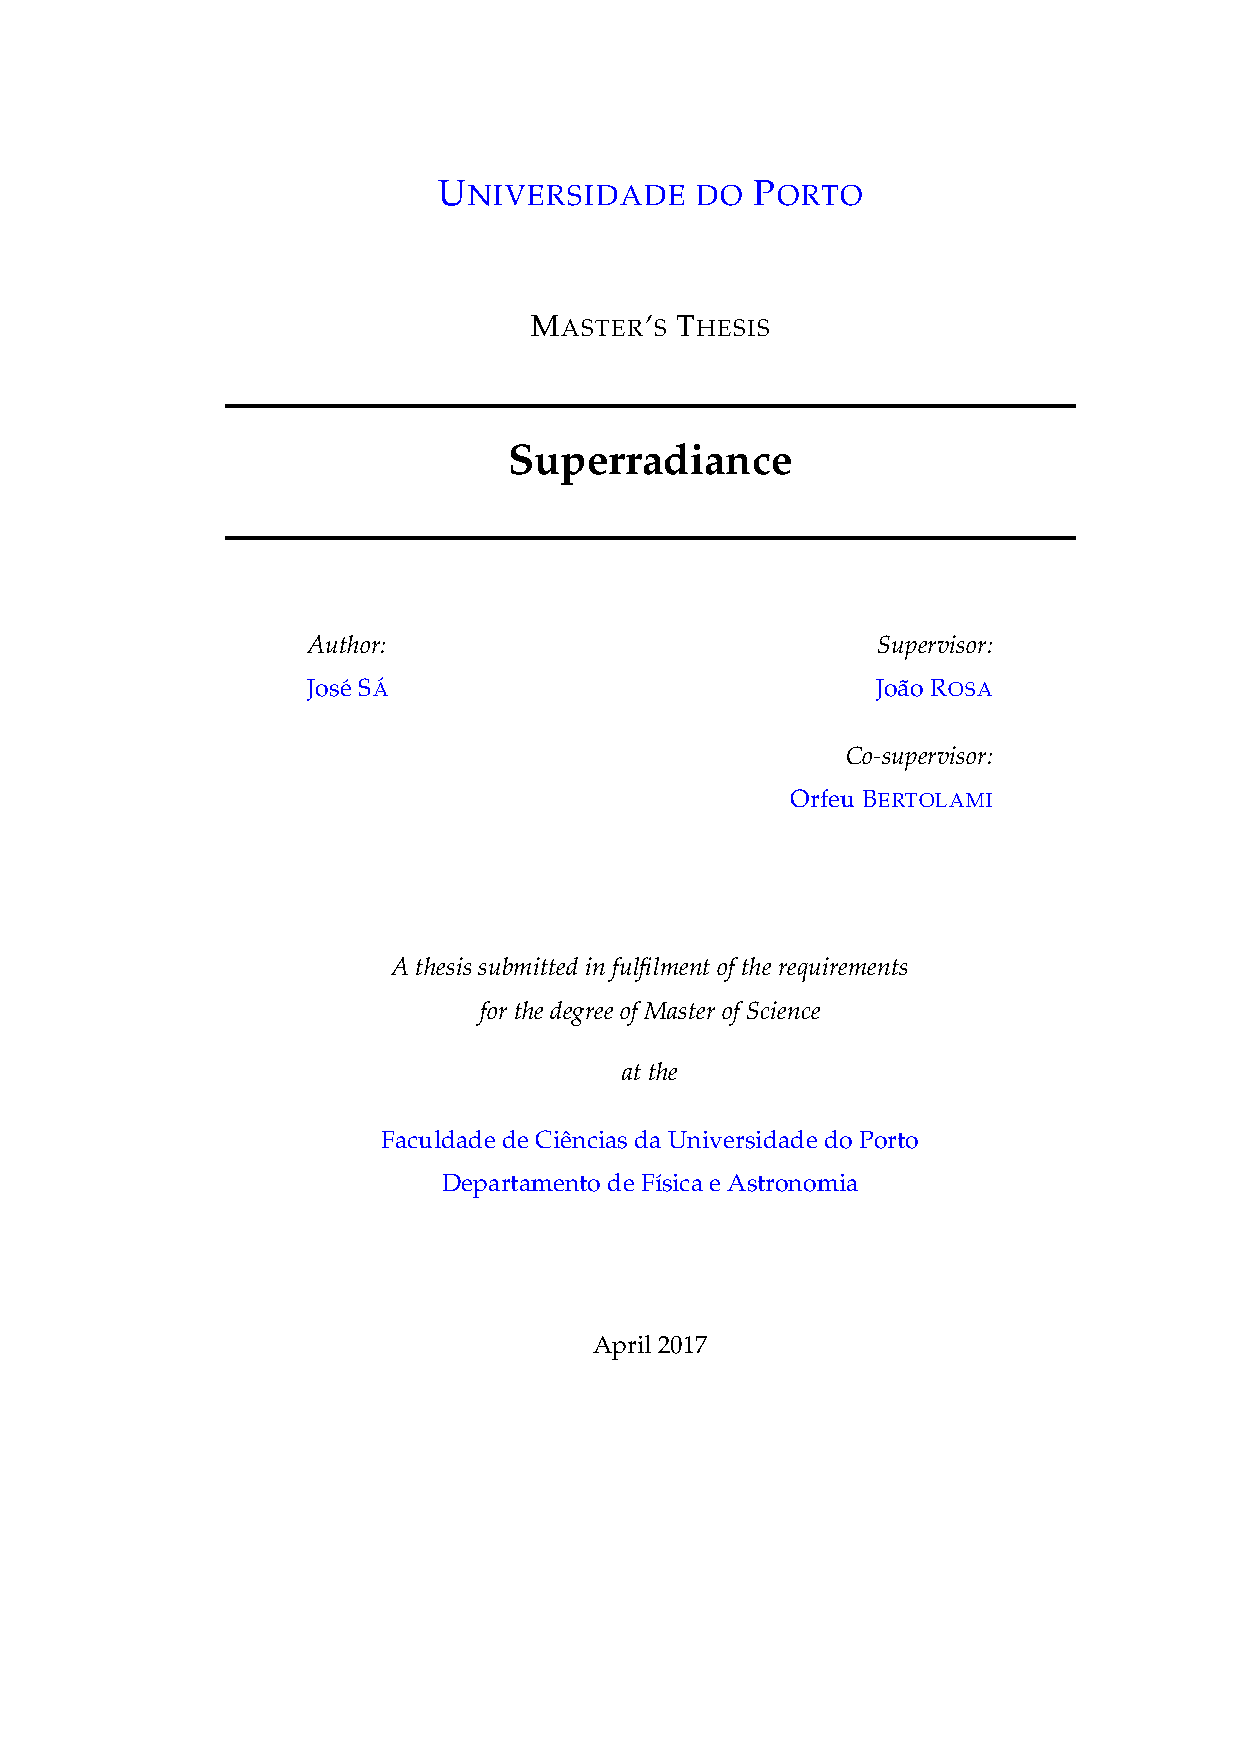
\includepdf[page={1},pagecommand={},scale=1]{Front/main}
\cleardoublepage
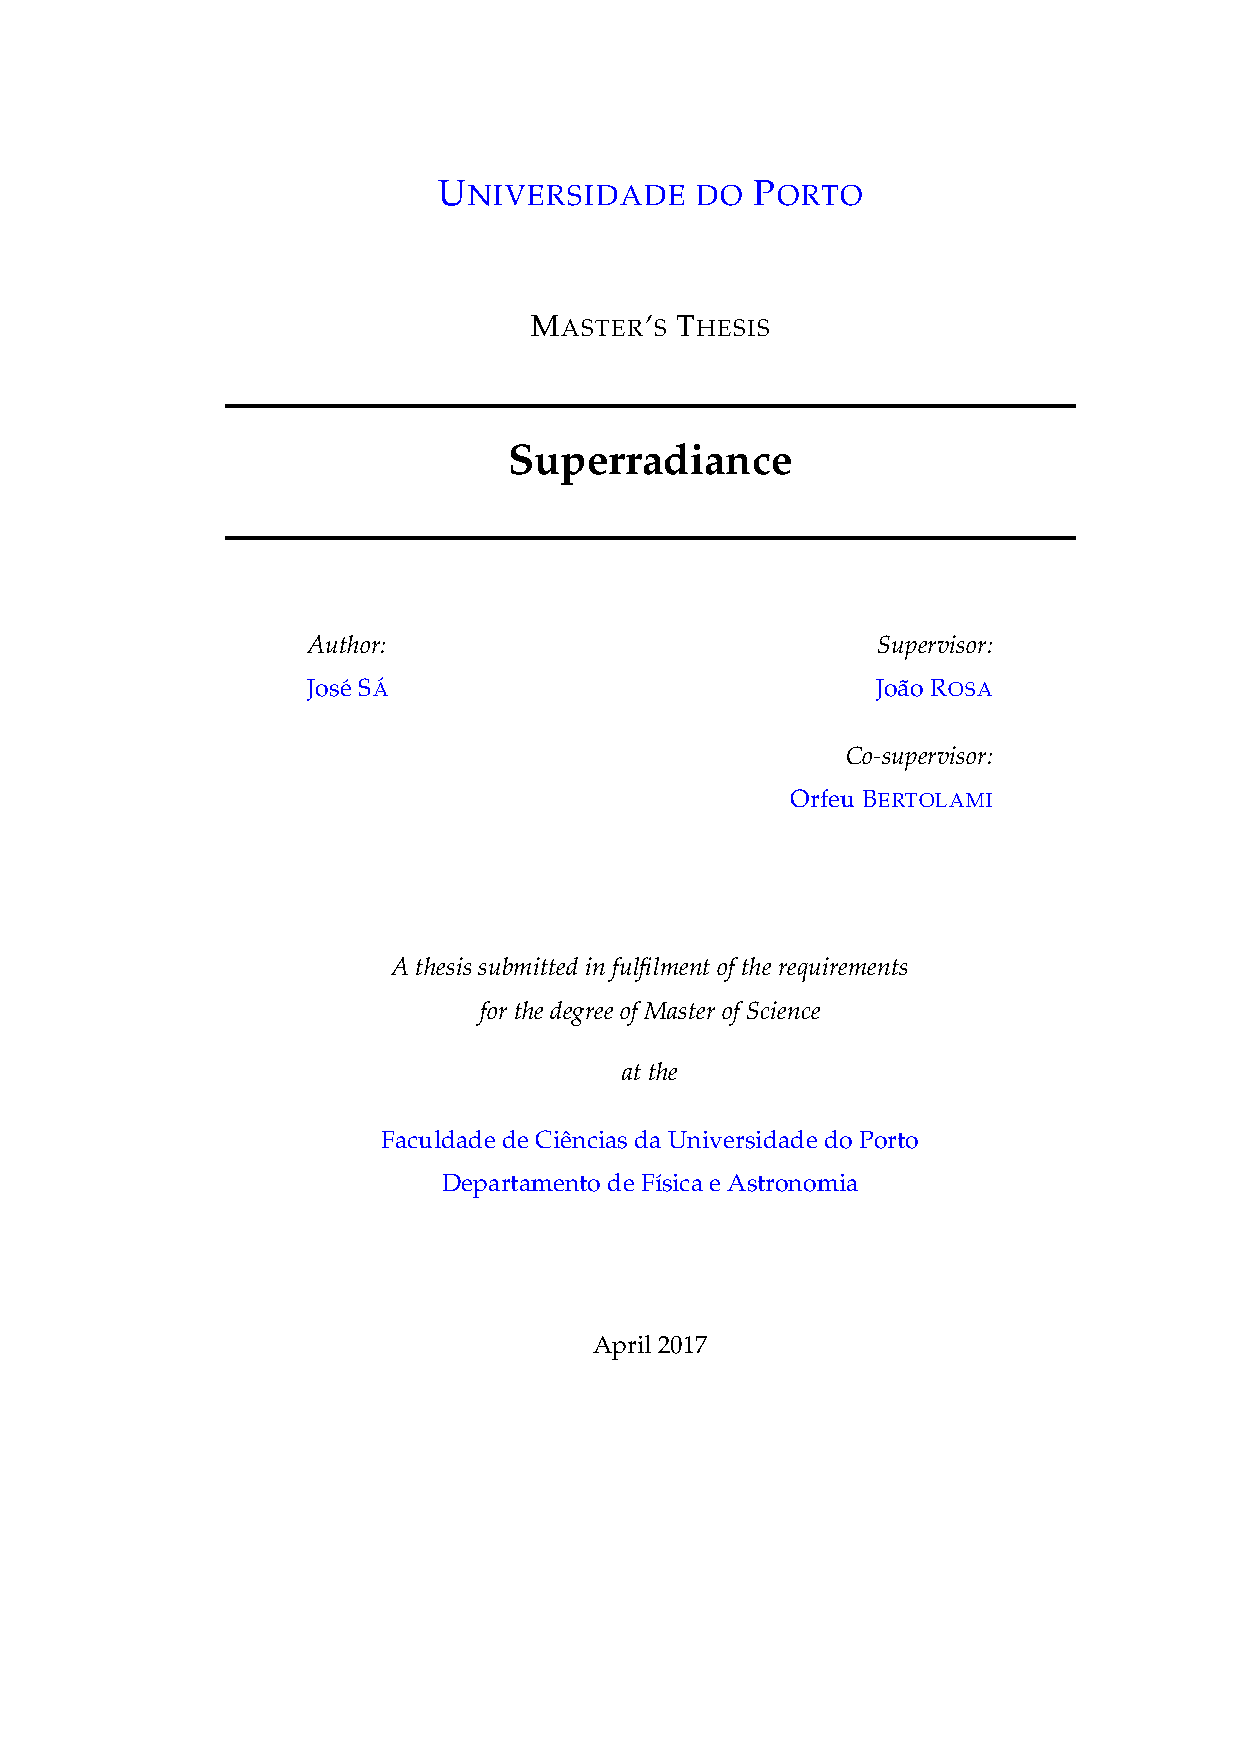
\includepdf[page={2},pagecommand={},scale=1]{Front/main}
\cleardoublepage
\pagestyle{fancy}


%----------------------------------------------------------------------------------------
%	TITLE PAGE
%----------------------------------------------------------------------------------------

\frontmatter % Use roman page numbering style (i, ii, iii, iv...) for the pre-content pages

\maketitle

 
%----------------------------------------------------------------------------------------
%	QUOTATION PAGE
%----------------------------------------------------------------------------------------

% \quotepage{author}
% {
% 	Quote \ldots
% }


%----------------------------------------------------------------------------------------
%	ACKNOWLEDGEMENTS
%----------------------------------------------------------------------------------------
%TC:break Acknowledgements

\begin{acknowledgements}
	\lipsum[1]
\end{acknowledgements}

\addvspacetoc{0.3cm} % Add a gap in the Contents, for aesthetics


%----------------------------------------------------------------------------------------
%	ABSTRACT PAGE
%----------------------------------------------------------------------------------------
%TC:break Abstract

\begin{abstract}
	The Thesis Abstract is written here (and usually kept to just this page). The page is kept centered vertically so can expand into the blank space above the title too\ldots	
\end{abstract}


%----------------------------------------------------------------------------------------
%	ABSTRACT PAGE (PORTUGUESE)
%----------------------------------------------------------------------------------------
%TC:break Resumo

\begin{abstract}[title={Resumo},degree={Mestre de Ciência},nameconnector={por}]
	Tradução em português do ``Abstract'' escrito em inglês mais a cima. A página é centrada vertical  e horizontalmente, podendo espandir para o espaço superior da página em branco \ldots
\end{abstract}


%----------------------------------------------------------------------------------------
%	LIST OF CONTENTS/FIGURES/TABLES
%----------------------------------------------------------------------------------------

\addvspacetoc{0.3cm}

\tableofcontents % Write out the Table of Contents

\listoffigures % Write out the List of Figures

\listoftables % Write out the List of Tables

\addvspacetoc{0.3cm}

%----------------------------------------------------------------------------------------
%	PHYSICAL CONSTANTS/OTHER DEFINITIONS
%----------------------------------------------------------------------------------------

% \begin{listofcontants}
% 	\const{My little ponny test of magical rainbow}{$mn/mp$}{$2.997\ 924\ 58\times10^{8}\ \mbox{ms}^{-\mbox{s}}$}
% 	\const{Vaccuum permeability test of magical rainbow for a specific case of condensed matter physics}{$\epsilon_0$}{$2.997\ 924\ 58\times10^{8}\ \mbox{ms}^{-\mbox{s}}$}
% 	\const{Speed of Light test of magical rainbow}{$c$}{$2.997\ 924\ 58\times10^{8}\ \mbox{ms}^{-\mbox{s}}$}
% 	\const{Speed of Light test of magical rainbow}{$c$}{$2.997\ 924\ 58\times10^{8}\ \mbox{ms}^{-\mbox{s}}$}
% \end{listofcontants}


%----------------------------------------------------------------------------------------
%	SYMBOLS
%----------------------------------------------------------------------------------------

% \begin{listofsymbols}
% 	\symb{$F_{\mu\nu}$}{Maxwell tensor}{F}
% 	\symb{$a$}{distance}{m}
% 	\\
% 	\symb{$\omega$}{angular frequency}{rads$^{-1}$}
% \end{listofsymbols}


%----------------------------------------------------------------------------------------
%	NOTATION
%----------------------------------------------------------------------------------------

\newcommand\notationname{Notation and Conventions}
\addtotoc{\notationname}
\fancyhead[LO]{\textsc{\notationname}}

% !TEX root = ../main.tex

\chapter*{Notation and Conventions}

\section*{Units}

Unit convetions

\section*{Tensors and GR related}

Metric definitions and stuff

\cleardoublepage



%----------------------------------------------------------------------------------------
%	ABBREVIATIONS
%----------------------------------------------------------------------------------------
%TC:break Glossary

\begin{glossary}
	\abbrev{BH}{Black Hole}
	\abbrev{BL}{Boyer-Linquist}
	\abbrev{EF}{Eddington-Finkelstein}
	\abbrev{GR}{General Relativity}
	\abbrev{GW}{Gravitational Wave}
%	\abbrev{KR}{Kerr-Newman}
	\abbrev{LIGO}{Laser Interferometric Gravitational Wave Observatory}
	\abbrev{NP}{Newman-Penrose}
%	\abbrev{QM}{Quantum Mechanics}
%	\abbrev{RN}{Reissner-Nordstr\"{o}m}
	\abbrev{SWSH}{Spin-Weighted Spheroidal Harmonic}
\end{glossary}


%----------------------------------------------------------------------------------------
%	DEDICATORY
%----------------------------------------------------------------------------------------

% \begin{dedicatory}
% 	For/Dedicated to/To my\ldots
% \end{dedicatory}


%----------------------------------------------------------------------------------------
%	THESIS CONTENT - CHAPTERS
%----------------------------------------------------------------------------------------

\addvspacetoc{0.3cm}

\mainmatter % Begin numeric (1,2,3...) page numbering

\pagestyle{fancy}
\renewcommand{\chaptermark}[1]{\markboth{\thechapter. \textsc{#1}}{}}
\fancyhead[LO]{\leftmark}


\chapter{Introduction} % Main chapter title
\label{Chapter1} 

%----------------------------------------------------------------------------------------

\section{Welcome and Thank You}
Welcome to this \LaTeX{} Thesis Template, a beautiful and easy to use template for writing a thesis using the \LaTeX{} typesetting system.

If you are writing a thesis (or will be in the future) and its subject is technical or mathematical (though it doesn't have to be), then creating it in \LaTeX{} is highly recommended as a way to make sure you can just get down to the essential writing without having to worry over formatting or wasting time arguing with your word processor.
\cite{Starobinsky1973}

\LaTeX{} is easily able to professionally typeset documents that run to hundreds or thousands of pages long. With simple mark-up commands, it automatically sets out the table of contents, margins, page headers and footers and keeps the formatting consistent and beautiful. One of its main strengths is the way it can easily typeset mathematics, even \emph{heavy} mathematics. Even if those equations are the most horribly twisted and most difficult mathematical problems that can only be solved on a super-computer, you can at least count on \LaTeX{} to make them look stunning.

%----------------------------------------------------------------------------------------

\section{Learning \LaTeX{}}

\LaTeX{} is not a WYSIWYG (What You See is What You Get) program, unlike word processors such as Microsoft Word or Apple's Pages. Instead, a document written for \LaTeX{} is actually a simple, plain text file that contains \emph{no formatting}. You tell \LaTeX{} how you want the formatting in the finished document by writing in simple commands amongst the text, for example, if I want to use \textit{italic text for emphasis}, I write the `$\backslash$\texttt{textit}\{\}' command and put the text I want in italics in between the curly braces. This means that \LaTeX{} is a ``mark-up'' language, very much like HTML.

\subsection{A (not so short) Introduction to \LaTeX{}}

If you are new to \LaTeX{}, there is a very good eBook -- freely available online as a PDF file -- called, ``The Not So Short Introduction to \LaTeX{}''. The book's title is typically shortened to just ``lshort''. You can download the latest version (as it is occasionally updated) from here:\\
\href{http://www.ctan.org/tex-archive/info/lshort/english/lshort.pdf}{\texttt{http://www.ctan.org/tex-archive/info/lshort/english/lshort.pdf}}

It is also available in several other languages. Find yours from the list on this page:\\
\href{http://www.ctan.org/tex-archive/info/lshort/}{\texttt{http://www.ctan.org/tex-archive/info/lshort/}}

It is recommended to take a little time out to learn how to use \LaTeX{} by creating several, small `test' documents. Making the effort now means you're not stuck learning the system when what you \emph{really} need to be doing is writing your thesis.

\subsection{A Short Math Guide for \LaTeX{}}

If you are writing a technical or mathematical thesis, then you may want to read the document by the AMS (American Mathematical Society) called, ``A Short Math Guide for \LaTeX{}''. It can be found online here:\\
\href{http://www.ams.org/tex/amslatex.html}{\texttt{http://www.ams.org/tex/amslatex.html}}\\
under the ``Additional Documentation'' section towards the bottom of the page.

\subsection{Common \LaTeX{} Math Symbols}
There are a multitude of mathematical symbols available for \LaTeX{} and it would take a great effort to learn the commands for them all. The most common ones you are likely to use are shown on this page:\\
\href{http://www.sunilpatel.co.uk/latexsymbols.html}{\texttt{http://www.sunilpatel.co.uk/latexsymbols.html}}

You can use this page as a reference or crib sheet, the symbols are rendered as large, high quality images so you can quickly find the \LaTeX{} command for the symbol you need.

\subsection{\LaTeX{} on a Mac}
 
The \LaTeX{} package is available for many systems including Windows, Linux and Mac OS X. The package for OS X is called MacTeX and it contains all the applications you need -- bundled together and pre-customised -- for a fully working \LaTeX{} environment and workflow.
 
MacTeX includes a dedicated \LaTeX{} IDE (Integrated Development Environment) called ``TeXShop'' for writing your `\texttt{.tex}' files and ``BibDesk'': a program to manage your references and create your bibliography section just as easily as managing songs and creating playlists in iTunes.

%----------------------------------------------------------------------------------------

\section{Getting Started with this Template}

If you are familiar with \LaTeX{}, then you can familiarise yourself with the contents of the Zip file and the directory structure and then place your own information into the `\texttt{Thesis.cls}' file. Section \ref{FillingFile} on page \pageref{FillingFile} tells you how to do this. Make sure you read section \ref{ThesisConventions} about thesis conventions to get the most out of this template and then get started with the `\texttt{Thesis.tex}' file straightaway.

If you are new to \LaTeX{} it is recommended that you carry on reading through the rest of the information in this document.

\subsection{About this Template}

This \LaTeX{} Thesis Template is originally based and created around a \LaTeX{} style file created by Steve R.\ Gunn from the University of Southampton (UK), department of Electronics and Computer Science. You can find his original thesis style file at his site, here:\\
\href{http://www.ecs.soton.ac.uk/~srg/softwaretools/document/templates/}{\texttt{http://www.ecs.soton.ac.uk/$\sim$srg/softwaretools/document/templates/}}

My thesis originally used the `\texttt{ecsthesis.cls}' from his list of styles. However, I knew \LaTeX{} could still format better. To get the look I wanted, I modified his style and also created a skeleton framework and folder structure to place the thesis files in.

This Thesis Template consists of that modified style, the framework and the folder structure. All the work that has gone into the preparation and groundwork means that all you have to bother about is the writing.

Before you begin using this template you should ensure that its style complies with the thesis style guidelines imposed by your institution. In most cases this template style and layout will be suitable. If it is not, it may only require a small change to bring the template in line with your institution's recommendations.

%----------------------------------------------------------------------------------------

\section{What this Template Includes}

\subsection{Folders}

This template comes as a single Zip file that expands out to many files and folders. The folder names are mostly self-explanatory:

\textbf{Appendices} -- this is the folder where you put the appendices. Each appendix should go into its own separate `\texttt{.tex}' file. A template is included in the directory.

\textbf{Chapters} -- this is the folder where you put the thesis chapters. A thesis usually has about seven chapters, though there is no hard rule on this. Each chapter should go in its own separate `\texttt{.tex}' file and they usually are split as:
\begin{itemize}
\item Chapter 1: Introduction to the thesis topic
\item Chapter 2: Background information and theory
\item Chapter 3: (Laboratory) experimental setup
\item Chapter 4: Details of experiment 1
\item Chapter 5: Details of experiment 2
\item Chapter 6: Discussion of the experimental results
\item Chapter 7: Conclusion and future directions
\end{itemize}
This chapter layout is specialised for the experimental sciences.

\textbf{Figures} -- this folder contains all figures for the thesis. These are the final images that will go into the thesis document.

\textbf{Primitives} -- this is the folder that contains scraps, particularly because one final image in the `Figures' folder may be made from many separate images and photos, these source images go here. This keeps the intermediate files separate from the final thesis figures.

\subsection{Files}

Included are also several files, most of them are plain text and you can see their contents in a text editor. Luckily, many of them are auxiliary files created by \LaTeX{} or BibTeX and which you don't need to bother about:

\textbf{Bibliography.bib} -- this is an important file that contains all the bibliographic information and references that you will be citing in the thesis for use with BibTeX. You can write it manually, but there are reference manager programs available that will create and manage it for you. Bibliographies in \LaTeX{} are a large subject and you may need to read about BibTeX before starting with this.

\textbf{Thesis.cls} -- this is an important file. It is the style file that tells \LaTeX{} how to format the thesis. You will also need to open this file in a text editor and fill in your own information (such as name, department, institution). Luckily, this is not too difficult and is explained in section \ref{FillingFile} on page \pageref{FillingFile}.

\textbf{Thesis.pdf} -- this is your beautifully typeset thesis (in the PDF file format) created by \LaTeX{}.

\textbf{Thesis.tex} -- this is an important file. This is the file that you tell \LaTeX{} to compile to produce your thesis as a PDF file. It contains the framework and constructs that tell \LaTeX{} how to layout the thesis. It is heavily commented so you can read exactly what each line of code does and why it is there. After you put your own information into the `\texttt{Thesis.cls}' file, go to this file and begin filling it in -- you have now started your thesis!

\textbf{vector.sty} -- this is a \LaTeX{} package, it tells \LaTeX{} how to typeset mathematical vectors. Using this package is very easy and you can read the documentation on the site (you just need to look at the `\texttt{vector.pdf}' file):\\
\href{http://www.ctan.org/tex-archive/macros/latex/contrib/vector/}{\texttt{http://www.ctan.org/tex-archive/macros/latex/contrib/vector/}}

\textbf{lstpatch.sty} -- this is a \LaTeX{} package required by this LaTeX template and is included as not all \TeX{} distributions have it installed by default. You do not need to modify this file.

Files that are \emph{not} included, but are created by \LaTeX{} as auxiliary files include:

\textbf{Thesis.aux} -- this is an auxiliary file generated by \LaTeX{}, if it is deleted \LaTeX{} simply regenerates it when you run the main `\texttt{.tex}' file.

\textbf{Thesis.bbl} -- this is an auxiliary file generated by BibTeX, if it is deleted, BibTeX simply regenerates it when you run the main tex file. Whereas the `\texttt{.bib}' file contains all the references you have, this `\texttt{.bbl}' file contains the references you have actually cited in the thesis and is used to build the bibliography section of the thesis.

\textbf{Thesis.blg} -- this is an auxiliary file generated by BibTeX, if it is deleted BibTeX simply regenerates it when you run the main `\texttt{.tex}' file.

\textbf{Thesis.lof} -- this is an auxiliary file generated by \LaTeX{}, if it is deleted \LaTeX{} simply regenerates it when you run the main `\texttt{.tex}' file. It tells \LaTeX{} how to build the `List of Figures' section.

\textbf{Thesis.log} -- this is an auxiliary file generated by \LaTeX{}, if it is deleted \LaTeX{} simply regenerates it when you run the main `\texttt{.tex}' file. It contains messages from \LaTeX{}, if you receive errors and warnings from \LaTeX{}, they will be in this `\texttt{.log}' file.

\textbf{Thesis.lot} -- this is an auxiliary file generated by \LaTeX{}, if it is deleted \LaTeX{} simply regenerates it when you run the main `\texttt{.tex}' file. It tells \LaTeX{} how to build the `List of Tables' section.

\textbf{Thesis.out} -- this is an auxiliary file generated by \LaTeX{}, if it is deleted \LaTeX{} simply regenerates it when you run the main `\texttt{.tex}' file.


So from this long list, only the files with the `\texttt{.sty}', `\texttt{.bib}', `\texttt{.cls}' and `\texttt{.tex}' extensions are the most important ones. The other auxiliary files can be ignored or deleted as \LaTeX{} and BibTeX will regenerate them.

%----------------------------------------------------------------------------------------

\section{Filling in the `\texttt{Thesis.cls}' File}\label{FillingFile}

You will need to personalise the thesis template and make it your own by filling in your own information. This is done by editing the `\texttt{Thesis.cls}' file in a text editor.

Open the file and scroll down, past all the `$\backslash$\texttt{newcommand}\ldots' items until you see the entries for `\texttt{University Name}', `\texttt{Department Name}', etc\ldots.

Fill out the information about your group and institution and ensure you keep to block capitals where it asks you to. You can also insert web links, if you do, make sure you use the full URL, including the `\texttt{http://}' for this.

The last item you should need to fill in is the Faculty Name (in block capitals). When you have done this, save the file and recompile `\texttt{Thesis.tex}'. All the information you filled in should now be in the PDF, complete with web links. You can now begin your thesis proper!

%----------------------------------------------------------------------------------------

\section{The `\texttt{Thesis.tex}' File Explained}

The \texttt{Thesis.tex} file contains the structure of the thesis. There are plenty of written comments that explain what pages, sections and formatting the \LaTeX{} code is creating. Initially there seems to be a lot of \LaTeX{} code, but this is all formatting, and it has all been taken care of so you don't have to do it.

Begin by checking that your information on the title page is correct. For the thesis declaration, your institution may insist on something different than the text given. If this is the case, just replace what you see with what is required.

Then comes a page which contains a funny quote. You can put your own, or quote your favourite scientist, author, person, etc\ldots Make sure to put the name of the person who you took the quote from.

Next comes the acknowledgements. On this page, write about all the people who you wish to thank (not forgetting parents, partners and your advisor/supervisor).

The contents pages, list of figures and tables are all taken care of for you and do not need to be manually created or edited. The next set of pages are optional and can be deleted since they are for a more technical thesis: insert a list of abbreviations you have used in the thesis, then a list of the physical constants and numbers you refer to and finally, a list of mathematical symbols used in any formulae. Making the effort to fill these tables means the reader has a one-stop place to refer to instead of searching the internet and references to try and find out what you meant by certain abbreviations or symbols.

The list of symbols is split into the Roman and Greek alphabets. Whereas the abbreviations and symbols ought to be listed in alphabetical order (and this is \emph{not} done automatically for you) the list of physical constants should be grouped into similar themes.

The next page contains a one line dedication. Who will you dedicate your thesis to?

Finally, there is the section where the chapters are included. Uncomment the lines (delete the `\texttt{\%}' character) as you write the chapters. Each chapter should be written in its own file and put into the `Chapters' folder and named `\texttt{Chapter1}', `\texttt{Chapter2}, etc\ldots Similarly for the appendices, uncomment the lines as you need them. Each appendix should go into its own file and placed in the `Appendices' folder.

After the preamble, chapters and appendices finally comes the bibliography. The bibliography style (called `\texttt{unsrtnat}') is used for the bibliography and is a fully featured style that will even include links to where the referenced paper can be found online. Do not under estimate how grateful you reader will be to find that a reference to a paper is just a click away. Of course, this relies on you putting the URL information into the BibTeX file in the first place.

%----------------------------------------------------------------------------------------

\section{Thesis Features and Conventions}\label{ThesisConventions}

To get the best out of this template, there are a few conventions that you may want to follow.

One of the most important (and most difficult) things to keep track of in such a long document as a thesis is consistency. Using certain conventions and ways of doing things (such as using a Todo list) makes the job easier. Of course, all of these are optional and you can adopt your own method.

\subsection{Printing Format}

This thesis template is designed for single sided printing as most theses are printed and bound this way. This means that the left margin is always wider than the right (for binding). Four out of five people will now judge the margins by eye and think, ``I never 
noticed that before.''.

The headers for the pages contain the page number on the right side (so it is easy to flick through to the page you want) and the chapter name on the left side.

The text is set to 11 point and a line spacing of 1.3. Generally, it is much more readable to have a smaller text size and wider gap between the lines than it is to have a larger text size and smaller gap. Again, you can tune the text size and spacing should you want or need to. The text size can be set in the options for the `$\backslash$\texttt{documentclass}' command at the top of the `\texttt{Thesis.tex}' file and the spacing can be changed by setting a different value in the `$\backslash$\texttt{setstretch}' commands (scattered throughout the `\texttt{Thesis.tex}' file).

\subsection{Using US Letter Paper}

The paper size used in the template is A4, which is a common -- if not standard -- size in Europe. If you are using this thesis template elsewhere and particularly in the United States, then you may have to change the A4 paper size to the US Letter size. Unfortunately, this is not as simple as replacing instances of `\texttt{a4paper}' with `\texttt{letterpaper}'.

This is because the final PDF file is created directly from the \LaTeX{} source using a program called `\texttt{pdfTeX}' and in certain conditions, paper size commands are ignored and all documents are created with the paper size set to the size stated in the configuration file for pdfTeX (called `\texttt{pdftex.cfg}').

What needs to be done is to change the paper size in the configuration file for \texttt{pdfTeX} to reflect the letter size. There is an excellent tutorial on how to do this here: \\
\href{http://www.physics.wm.edu/~norman/latexhints/pdf_papersize.html}{\texttt{http://www.physics.wm.edu/$\sim$norman/latexhints/pdf\_papersize.html}}

It may be sufficient just to replace the dimensions of the A4 paper size with the US Letter size in the \texttt{pdftex.cfg} file. Due to the differences in the paper size, the resulting margins may be different to what you like or require (as it is common for Institutions to dictate certain margin sizes). If this is the case, then the margin sizes can be tweaked by opening up the \texttt{Thesis.cls} file and searching for the line beginning with, `$\backslash$\texttt{setmarginsrb}' (not very far down from the top), there you will see the margins specified. Simply change those values to what you need (or what looks good) and save. Now your document should be set up for US Letter paper size with suitable margins.

\subsection{References}

The `\texttt{natbib}' package is used to format the bibliography and inserts references such as this one. The options used in the `\texttt{Thesis.tex}' file mean that the references are listed in numerical order as they appear in the text. Multiple references are rearranged in numerical order and multiple, sequential references become reformatted to a reference range. This is done automatically for you. To see how you use references, have a look at the `\texttt{Chapter1.tex}' source file. Many reference managers allow you to simply drag the reference into the document as you type.

Scientific references should come \emph{before} the punctuation mark if there is one (such as a comma or period). The same goes for footnotes\footnote{Such as this footnote, here down at the bottom of the page.}. You can change this but the most important thing is to keep the convention consistent throughout the thesis. Footnotes themselves should be full, descriptive sentences (beginning with a capital letter and ending with a full stop).

To see how \LaTeX{} typesets the bibliography, have a look at the very end of this document (or just click on the reference number links).

\subsection{Figures}

There will hopefully be many figures in your thesis (that should be placed in the `Figures' folder). The way to insert figures into your thesis is to use a code template like this:
\begin{verbatim}
\begin{figure}[htbp]
  \centering
    
\includegraphics{Figures/Electron.pdf}
    \rule{35em}{0.5pt}
  \caption[An Electron]{An electron (artist's impression).}
  \label{fig:Electron}
\end{figure}
\end{verbatim}
Also look in the source file. Putting this code into the source file produces the picture of the electron that you can see in the figure below.

\begin{figure}[htbp]
	\centering
		
\includegraphics{Figures/Electron.pdf}
		\rule{35em}{0.5pt}
	\caption[An Electron]{An electron (artist's impression).}
	\label{fig:Electron}
\end{figure}

Sometimes figures don't always appear where you write them in the source. The placement depends on how much space there is on the page for the figure. Sometimes there is not enough room to fit a figure directly where it should go (in relation to the text) and so \LaTeX{} puts it at the top of the next page. Positioning figures is the job of \LaTeX{} and so you should only worry about making them look good!

Figures usually should have labels just in case you need to refer to them (such as in Figure \ref{fig:Electron}). The `$\backslash$\texttt{caption}' command contains two parts, the first part, inside the square brackets is the title that will appear in the `List of Figures', and so should be short. The second part in the curly brackets should contain the longer and more descriptive caption text.

The `$\backslash$\texttt{rule}' command is optional and simply puts an aesthetic horizontal line below the image. If you do this for one image, do it for all of them.

The \LaTeX{} Thesis Template is able to use figures that are either in the PDF or JPEG file format.

\subsection{Typesetting mathematics}

If your thesis is going to contain heavy mathematical content, be sure that \LaTeX{} will make it look beautiful, even though it won't be able to solve the equations for you.

The ``Not So Short Introduction to \LaTeX{}'' (available \href{http://www.ctan.org/tex-archive/info/lshort/english/lshort.pdf}{here}) should tell you everything you need to know for most cases of typesetting mathematics. If you need more information, a much more thorough mathematical guide is available from the AMS called, ``A Short Math Guide to \LaTeX{}'' and can be downloaded from:\\
\href{ftp://ftp.ams.org/pub/tex/doc/amsmath/short-math-guide.pdf}{\texttt{ftp://ftp.ams.org/pub/tex/doc/amsmath/short-math-guide.pdf}}

There are many different \LaTeX{} symbols to remember, luckily you can find the most common symbols \href{http://www.sunilpatel.co.uk/latexsymbols.html}{here}. You can use the web page as a quick reference or crib sheet and because the symbols are grouped and rendered as high quality images (each with a downloadable PDF), finding the symbol you need is quick and easy.

You can write an equation, which is automatically given an equation number by \LaTeX{} like this:
\begin{verbatim}
\begin{equation}
E = mc^{2}
  \label{eqn:Einstein}
\end{equation}
\end{verbatim}

This will produce Einstein's famous energy-matter equivalence equation:
\begin{equation}
E = mc^{2}
\label{eqn:Einstein}
\end{equation}

All equations you write (which are not in the middle of paragraph text) are automatically given equation numbers by \LaTeX{}. If you don't want a particular equation numbered, just put the command, `$\backslash$\texttt{nonumber}' immediately after the equation.

%----------------------------------------------------------------------------------------

\section{Sectioning and Subsectioning}

You should break your thesis up into nice, bite-sized sections and subsections. \LaTeX{} automatically builds a table of Contents by looking at all the `$\backslash$\texttt{chapter}$\{\}$', `$\backslash$\texttt{section}$\{\}$' and `$\backslash$\texttt{subsection}$\{\}$' commands you write in the source.

The table of Contents should only list the sections to three (3) levels. A `$\backslash$\texttt{chapter}$\{\}$' is level one (1). A `$\backslash$\texttt{section}$\{\}$' is level two (2) and so a `$\backslash$\texttt{subsection}$\{\}$' is level three (3). In your thesis it is likely that you will even use a `$\backslash$\texttt{subsubsection}$\{\}$', which is level four (4). Adding all these will create an unnecessarily cluttered table of Contents and so you should use the `$\backslash$\texttt{subsubsection$^{*}\{\}$}' command instead (note the asterisk). The asterisk ($^{*}$) tells \LaTeX{} to omit listing the subsubsection in the Contents, keeping it clean and tidy.

%----------------------------------------------------------------------------------------

\section{In Closing}

You have reached the end of this mini-guide. You can now rename or overwrite this pdf file and begin writing your own `\texttt{Chapter1.tex}' and the rest of your thesis. The easy work of setting up the structure and framework has been taken care of for you. It's now your job to fill it out!

\lipsum[20]

Good luck and have lots of fun!

\cleardoublepage

% Chapter Template

\chapter{Mathematical preliminaries} % Main chapter title
\label{Chapter2}


%----------------------------------------------------------------------------------------
%	SECTION 1
%----------------------------------------------------------------------------------------

\section{Tetrad formalism}

Lorem ipsum dolor sit amet, consectetur adipiscing elit. Aliquam ultricies lacinia euismod. Nam tempus risus in dolor rhoncus in interdum enim tincidunt. Donec vel nunc neque. In condimentum ullamcorper quam non consequat. Fusce sagittis tempor feugiat. Fusce magna erat, molestie eu convallis ut, tempus sed arcu. Quisque molestie, ante a tincidunt ullamcorper, sapien enim dignissim lacus, in semper nibh erat lobortis purus. Integer dapibus ligula ac risus convallis pellentesque.

%-----------------------------------
%	SUBSECTION 1
%-----------------------------------
\subsection{Subsection 1}

Nunc posuere quam at lectus tristique eu ultrices augue venenatis. Vestibulum ante ipsum primis in faucibus orci luctus et ultrices posuere cubilia Curae; Aliquam erat volutpat. Vivamus sodales tortor eget quam adipiscing in vulputate ante ullamcorper. Sed eros ante, lacinia et sollicitudin et, aliquam sit amet augue. In hac habitasse platea dictumst.

%-----------------------------------
%	SUBSECTION 2
%-----------------------------------

\subsection{Subsection 2}
Morbi rutrum odio eget arcu adipiscing sodales. Aenean et purus a est pulvinar pellentesque. Cras in elit neque, quis varius elit. Phasellus fringilla, nibh eu tempus venenatis, dolor elit posuere quam, quis adipiscing urna leo nec orci. Sed nec nulla auctor odio aliquet consequat.
Ut nec nulla in ante ullamcorper aliquam at sed dolor. Phasellus fermentum magna in augue gravida cursus. Cras sed pretium lorem. Pellentesque eget ornare odio. Proin accumsan, massa viverra cursus pharetra, ipsum nisi lobortis velit, a malesuada dolor lorem eu neque.

%----------------------------------------------------------------------------------------
%	SECTION 2
%----------------------------------------------------------------------------------------

\section{Newman-Penrose formalism}

Sed ullamcorper quam eu nisl interdum at interdum enim egestas. Aliquam placerat justo sed lectus lobortis ut porta nisl porttitor. Vestibulum mi dolor, lacinia molestie gravida at, tempus vitae ligula. Donec eget quam sapien, in viverra eros. Donec pellentesque justo a massa fringilla non vestibulum metus vestibulum. Vestibulum in orci quis felis tempor lacinia. Vivamus ornare ultrices facilisis. Ut hendrerit volutpat vulputate. Morbi condimentum venenatis augue, id porta ipsum vulputate in. Curabitur luctus tempus justo. Vestibulum risus lectus, adipiscing nec condimentum quis, condimentum nec nisl. Aliquam dictum sagittis velit sed iaculis. Morbi tristique augue sit amet nulla pulvinar id facilisis ligula mollis. Nam elit libero, tincidunt ut aliquam at, molestie in quam. Aenean rhoncus vehicula hendrerit. 
% !TEX root = ../Main.tex

\chapter{Teukolsky's master equation} % Main chapter title
\label{Chapter3}

%-----------------------------------------------------------------------------------

\section{Newman-Penrose formalism}

The study of gravitational and electromagnetic perturbations in a BH background was performed long before Kerr found his solution, for other spacetimes such as Schwarzschild's.
Despite its simplicity, the procedure involved was already algebraically tedious.
In the Kerr case, the metric was far more complicated, making the problem almost untreatable.

Fortunately, the NP formalism \cite{Newman1962} provides an alternative method of studying perturbations.
This formalism results from a natural introduction of spinor techniques in GR, after the choice of a null complex tetrad basis,
\begin{align}
    \bm{e}_a = (e_a)^\mu \frac{\partial}{\partial x^\mu} \qquad (a = 1, 2, 3, 4) ~,
\end{align}
where all quantities will be projected, \emph{i.e.} for the Weyl tensor we define
\begin{align}
    C_{abcd} =  (e_a)^\alpha \,(e_b)^\beta \,(e_c)^\gamma \,(e_d)^\delta \,C_{\alpha\beta\gamma\delta} ~.
\end{align}
Penrose believed that the light-cone was the essential element of the spacetime, thus it was of importance to find null directions.
The basis consisted in two real vectors, $\bm{\mathfrak{l}}$ and $\bm{\mathfrak{n}}$, and two complex conjugate vectors $\bm{\mathfrak{m}}$ and $\bar{\bm{\mathfrak{m}}}$.
Besides satisfying
\begin{align}
    \bm{\mathfrak{l}}^2 = \bm{\mathfrak{n}}^2 = \bm{\mathfrak{m}}^2 = \bar{\bm{\mathfrak{m}}}^2 = 0 ~,
\end{align}
orthogonality conditions of NP formalism require
\begin{align}
   \bm{\mathfrak{l}} \cdot \bm{\mathfrak{m}} = \bm{\mathfrak{l}} \cdot \bar{\bm{\mathfrak{m}}} = \bm{\mathfrak{n}} \cdot \bm{\mathfrak{m}} = \bm{\mathfrak{n}} \cdot \bar{\bm{\mathfrak{m}}} = 0 ~.
\end{align}
Still we are left with the ambiguity raised by multiplication of scalar functions to each vector, therefore it is customary to impose normalization conditions to the basis,
\begin{align}
    \bm{\mathfrak{l}} \cdot \bm{\mathfrak{n}} = 1 ~, \qquad \bm{\mathfrak{m}} \cdot \bar{\bm{\mathfrak{m}}} = -1 ~.
\end{align}
This formalism is a special case of tetrad calculus, where we can identify the new basis as $(\bm{\mathfrak{l}},\bm{\mathfrak{n}},\bm{\mathfrak{m}},\bar{\bm{\mathfrak{m}}})$. The ``metric'' for manipulating tetrad indices, $\eta_{ab}$, is defined by all restrictions provided above,
\begin{align}
    g^{\mu\nu} = \eta^{ab} (e_a)^\mu (e_b)^\nu = \mathfrak{l}^{\mu} \mathfrak{n}^{\nu} + \mathfrak{n}^{\mu} \mathfrak{l}^{\nu} - \mathfrak{m}^{\mu} \bar{\mathfrak{m}}^{\nu} - \bar{\mathfrak{m}}^{\mu} \mathfrak{m}^{\nu} ~.
\end{align}
Additionally these vectors define new directional derivatives.
We will depart shortly from standard notation, by redefining these derivatives as
\begin{align}
    \mathbbl{D}=\nabla_{\bm{\mathfrak{l}}} ~,\qquad \mathbbl{\Delta}=\nabla_{\bm{\mathfrak{n}}} ~,\qquad \bbdelta=\nabla_{\bm{\mathfrak{m}}} ~,\qquad \bar{\bbdelta}=\nabla_{\bar{\bm{\mathfrak{m}}}} ~.
    \label{eq3:tetradCovDer}
\end{align}

More details and definitions on the tetrad formalism can be found in~\aref{AppendixTetradFormalism}.

%-----------------------------------------------------------------------------------

\subsection{Kinnersley tetrad}

The Riemann tensor may have up to twenty non-vanishing components.
We know that ten of these are present in the symmetric Ricci tensor, that is intrinsically connected to matter and energy.
The other components are pure gravitational degrees of freedom and are encoded in the Weyl tensor.
It becomes the most useful object when the Ricci tensor vanishes, such as for vacuum solutions and source-free gravitational waves.
In order to remove the Ricci tensor degrees of freedom, the tensor must be constructed as trace-free,
\begin{align}
    \eta^{ad} C_{abcd} = C_{1bc2} + C_{1bc2} - C_{3bc4} - C_{4bc3} = 0 ~. 
\end{align}
Together with the other symmetries inherited from the Riemann tensor, for instance the first Bianchi identity, $C_{a[bcd]}=0$, it is possible to show that some of these NP components vanish while others remain related, leaving us with ten degrees of freedom.
As a result, in the NP formalism the Weyl tensor can be represented by five complex scalars, usually chosen as
\begin{align}
    \begin{split}
        \psi_0 &= - C_{1313} = - C_{\alpha\beta\gamma\delta}\, \mathfrak{l}^\alpha \mathfrak{m}^\beta \mathfrak{l}^\gamma \mathfrak{m}^\delta ~,\qquad
        ~\psi_1 = - C_{1213} = - C_{\alpha\beta\gamma\delta}\, \mathfrak{l}^\alpha \mathfrak{n}^\beta \mathfrak{l}^\gamma \mathfrak{m}^\delta ~,\\
        \psi_2 &= - C_{1342} = - C_{\alpha\beta\gamma\delta}\, \mathfrak{l}^\alpha \mathfrak{m}^\beta \bar{\mathfrak{m}}^\gamma \mathfrak{n}^\delta ~,\qquad
        \psi_3 = - C_{1242} = - C_{\alpha\beta\gamma\delta}\, \mathfrak{l}^\alpha \mathfrak{n}^\beta \bar{\mathfrak{m}}^\gamma \mathfrak{n}^\delta ~,\\
        \psi_4 &= - C_{2424} = - C_{\alpha\beta\gamma\delta}\, \mathfrak{n}^\alpha \bar{\mathfrak{m}}^\beta \mathfrak{n}^\gamma \bar{\mathfrak{m}}^\delta ~.
    \end{split}
\end{align}
The complex conjugates can be obtained by doing the replacement $3 \rightleftarrows 4$, by exchanging $\bm{\mathfrak{m}}$ with $\bar{\bm{\mathfrak{m}}}$ and vice-versa. 
The Weyl tensor has a unique decomposition in terms of a linear combination of NP scalars and tensorial product of two-forms.
This decomposition has the general form,
\begin{align}
    \begin{split}
    \frac{1}{4} \, C_{\mu\nu\rho\sigma} = & - \psi_0 \,V_{\mu\nu} V_{\rho\sigma} - \psi_1 \, (V_{\mu\nu} W_{\rho\sigma} + W_{\mu\nu} V_{\rho\sigma}) \\
    & - \psi_2 \, (U_{\mu\nu}V_{\rho\sigma} + V_{\mu\nu}U_{\rho\sigma} + W_{\mu\nu}W_{\rho\sigma}) \\
    & - \psi_3 \, (U_{\mu\nu}W_{\rho\sigma} + W_{\mu\nu}U_{\rho\sigma})
    - \psi_4 \, U_{\mu\nu}U_{\rho\sigma} + \text{ c.c.}
    \end{split}
\end{align}
where $U_{\mu\nu} = \mathfrak{l}_{[\mu} \mathfrak{m}_{\nu]}$, $V_{\mu\nu} = \bar{\mathfrak{m}}_{[\mu} \mathfrak{n}_{\nu]}$, $W_{\mu\nu} = \mathfrak{l}_{[\mu} \mathfrak{n}_{\nu]} - \mathfrak{m}_{[\mu} \bar{\mathfrak{m}}_{\nu]}$.
It is clear that the values that these five complex scalars take is completely dependent on the choice of tetrad frame. 

BH solutions are ``type D'' spacetimes according to Petrov's classification, which was a major restriction necessary to the discovery of Kerr's metric.
For these spacetimes it is possible to find two different doubly-degenerate principal directions of the Weyl tensor, which we choose to be the real vectors of the tetrad, $\bm{\mathfrak{l}}$ and $\bm{\mathfrak{n}}$ \cite{Chandrasekhar1998}.
These yield
\begin{align}
    C_{\mu\alpha\beta[\nu} \mathfrak{l}_{\rho]} \mathfrak{l}^\alpha \mathfrak{l}^\beta = 0 ~, \qquad C_{\mu\alpha\beta[\nu} \mathfrak{n}_{\rho]} \mathfrak{n}^\alpha \mathfrak{n}^\beta = 0  ~.
\end{align}
In NP formalism terms, this implies, respectively,
\begin{align}
    \psi_0=\psi_1=0 ~,\qquad \psi_3=\psi_4=0 ~.
\end{align}

Finding the principal directions may not be trivial, but we can apply successive local transformations of the six-parameter Lorentz group in order to rotate the tetrad vectors. 
This procedure allows for the simplification of the Weyl tensor by vanishing NP scalars, ``locking'' the orientation of the tetrad frame.
The Weyl scalar $\psi_2$ becomes invariant under boosts in the principal directions, usually refereed as ``type III'' rotations \cite{Chandrasekhar1998}.
These keep the light-cone structure intact by maintaining the direction of $\bm{\mathfrak{l}}$ and $\bm{\mathfrak{n}}$ unchanged (up to multiplication of scalar functions), being useful to change between ingoing and outgoing frames \cite{Teukolsky1974}. 
Kinnersly solved the type D vacuum field equations \cite{Kinnersley1969}, finding a suitable tetrad 
\begin{align}
    \label{eq3:kinnerslytetrad}
    \begin{split}
        \bm{\mathfrak{l}} =& \left(\frac{r^2+a^2}{\Delta}, \, 1, \,0, \,\frac{a}{\Delta} \right) ~, \\
        \bm{\mathfrak{n}} =& \frac{1}{2 \rho^2} \Bigr( r^2+a^2, \,-\Delta, \,0 , \,a \Bigr) ~, \\
        \bm{\mathfrak{m}} =& \frac{1}{ \sqrt{2} \bar{\rho}^2 } \Bigr( i a \sin\theta, \,0, \,1, \, i \csc\theta \Bigr) ~,
    \end{split}
\end{align}
where $\bar{\rho} = r + i a \cos\theta$ and $\rho^2 \equiv | \bar{\rho} |^2 = \bar{\rho} \bar{\rho}^*$.

The NP formalism provides a full set of first-order coupled differential equations, relating the NP scalars components of the Weyl and Maxwell tensors. 
These equations result from the second Bianchi identity, $C_{\mu\nu[\rho \sigma ; \lambda ]} = 0$, and the Maxwell equations.
In order to write these equations explicitly we need to define the \emph{spin coefficients} using the connection $\gamma_{abc} = (e_{a})^\mu (e_{b})_{\mu;\nu} (e_{c})^\nu$, which replaces the Christopher symbols in this formalism.

To study GWs, instead of perturbing the background metric, the NP formalism provides a natural way of performing perturbations by modification of the tetrad, $\bm{\mathfrak{l}}=\bm{\mathfrak{l}}^B+\bm{\mathfrak{l}}^P$, $\bm{\mathfrak{n}}=\bm{\mathfrak{n}}^B+\bm{\mathfrak{n}}^P$, etc., and also the NP scalars, $\psi_a = \psi_a{}^B + \psi_a{}^P$, maintaining only first-order terms \cite{Teukolsky1973a}.
The formalism reveals decoupled equations for $\psi_0{}^P$ and $\psi_4{}^P$, which implies that these dynamic variables are the only independent degrees of freedom of the GWs.

%-----------------------------------------------------------------------------------

\subsection{Maxwell equations}

We focus with more detail on EM perturbations with a fixed background because they involve a simpler procedure and then we will tie with the same master equation that also describes GW perturbations. 
 
In the NP formalism, all Maxwell equations, $F_{[\mu\nu; \rho]}=0$ and \eqref{eq2:maxwellEM}, reduce to
\begin{align}
    \label{eq3:maxwellFabEqs}
    F_{[ab \rvert c]} = 0 ~,\qquad \eta^{bc} F_{ab \rvert c} = 0 ~
\end{align}
(see \aref{AppendixTetradFormalism}).
The Maxwell tensor $F_{\mu\nu}$ has a total of six components which encodes the vector quantities of the electric and the magnetic fields. We may reduce the equation using three complex NP scalars,
\begin{align}
    \label{eq3:maxwellNPphi}
    \begin{split}
        \phi_0 &= F_{13} = F_{\alpha\beta} \,\mathfrak{l}^\alpha \mathfrak{m}^\beta ~,\\
        \phi_1 &= \tfrac{1}{2} (F_{12} + F_{43}) = \tfrac{1}{2} F_{\alpha\beta} \,(\mathfrak{l}^\alpha \mathfrak{n}^\beta + \bar{\mathfrak{m}}^\alpha \mathfrak{m}^\beta) ~,\\
        \phi_2 &= F_{42} = F_{\alpha\beta} \,\bar{\mathfrak{m}}^\alpha \mathfrak{n}^\beta ~.
    \end{split}
\end{align}
%$\tfrac{1}{2} F_{\mu\nu} = - \phi_0 \,V_{\mu\nu} - \phi_1 \,W_{\mu\nu} - \phi_2 \,U_{\mu\nu}+ \text{ c.c.}$
Considering all possible combinations of NP indices in \eref{eq3:maxwellFabEqs}, we gather eight equations, double the amount of necessary relations. 
This occurs because the conjugates $\phi_0^*$, $\phi_1^*$, $\phi_2^*$ are coupled in these equations. Eliminating every term of the form $F_{23\rvert a}$ or $F_{14\rvert b}$, 
\begin{subequations}
    \begin{align}
        \phi_{2\rvert 1} &= \phi_{1\rvert 4} ~, \label{eq3:phi21phi14}\\
        \phi_{1\rvert 2} &= \phi_{2\rvert 3} ~, \label{eq3:phi12phi23}\\
        \phi_{1\rvert 1} &= \phi_{0\rvert 4} ~, \label{eq3:phi11phi04}\\
        \phi_{0\rvert 2} &= \phi_{1\rvert 3} ~. \label{eq3:phi02phi13}
    \end{align}
\end{subequations}
We may expand explicitly the left-hand side of \eqref{eq3:phi21phi14},
\begin{align}
    \label{eq3:phi21SpinCoef}
    \begin{split}
        \phi_{2\rvert 1} &= \phi_{2, 1} - \eta^{ab}( \gamma_{a41} F_{b2} + \gamma_{a21} F_{4b} ) \\
        &= \phi_{2, 1} - (\gamma_{241} F_{12} + \gamma_{121} F_{42}) + ( \gamma_{341} F_{42} + \gamma_{421} F_{43} ) \\
        &= \phi_{2, 1} + 2 F_{42} \left(\frac{\gamma_{341} + \gamma_{211}}{2}\right) + 2 \gamma_{421} \left(\frac{F_{12} + F_{43}}{2}\right) \\
        &= \mathbbl{D} \phi_2 + 2 \varepsilon \phi_2 - 2 \pi \phi_1 ~,
    \end{split}
\end{align}
where we used the antisymmetry of the spin connection, $\gamma_{abc}=-\gamma_{bac}$. The right-hand side yields
\begin{align}
    \label{eq3:phi14SpinCoef}
    \begin{split}
        \phi_{1\rvert 4} &= \phi_{1, 4} - \tfrac{1}{2} \eta^{ab}( \gamma_{a14} F_{b2} + \gamma_{a24} F_{1b} + \gamma_{a44} F_{b3} + \gamma_{a34} F_{4b} ) \\
        &= \phi_{1, 4} - \tfrac{1}{2} ( \gamma_{144} F_{23} + \gamma_{134} F_{42} + \gamma_{214} F_{12} + \gamma_{234} F_{41} ) \\ 
        &\qquad\qquad + \tfrac{1}{2} ( \gamma_{314} F_{42} + \gamma_{414} F_{42} + \gamma_{324} F_{14} + \gamma_{424} F_{13} ) \\
        &= \phi_{2, 1} - \gamma_{244} F_{13} + \gamma_{314} F_{42} \\
        &= \bar{\bbdelta} \phi_1 - \lambda \phi_0 + \tau \phi_2  ~.
    \end{split}
\end{align}
The spin coefficients $\varepsilon$, $\pi$, $\lambda$, $\tau$, along with other NP definitions are found in~\aref{AppendixNPSpinCoef}. If we repeat the same expansion for the other Maxwell equations, we gather the set
\begin{subequations}
    \begin{align}
        \label{eq3:phi21phi14SpinCoef}
        \mathbbl{D} \phi_2 - \bar{\bbdelta} \phi_1 &= -\lambda \phi_0 + 2 \pi \phi_1 + (\varrho - 2 \varepsilon) \phi_2 ~,\\
        \label{eq3:phi12phi23SpinCoef}
        \mathbbl{\Delta} \phi_1 - \bbdelta \phi_2 &= \nu \phi_0 - 2 \mu \phi_1 + (2\beta-\tau) \phi_2 ~,\\
        \label{eq3:phi11phi04SpinCoef}
        \mathbbl{D} \phi_1 - \bar{\bbdelta} \phi_0 &= (\pi - 2 \alpha) \phi_0 + 2 \varrho \phi_1 - \kappa \phi_2 ~,\\
        \label{eq3:phi02phi13SpinCoef}
        \mathbbl{\Delta} \phi_0 - \bbdelta \phi_1 &= (2 \gamma - \mu) \phi_0 - 2 \tau \phi_1 + \sigma \phi_2 ~.
    \end{align}
\end{subequations}
The Kinnersley tetrad guarantees that $\kappa = \sigma = \lambda = \nu = 0$, decoupling all equations above. After substitution of all spin coefficients,
\begin{subequations}
    \begin{align}
        \label{eq3:phi21phi14Expand}
        \left( \mathbbl{D} + \frac{1}{\bar{\rho}^*} \right) \phi_2 &= 
        \left( \bar{\bbdelta} + \frac{2 i a \sin\theta}{\sqrt{2} (\bar{\rho}^*)^2} \right) \phi_2 ~,\\
        \label{eq3:phi12phi23Expand}
        \left( \mathbbl{\Delta} - \frac{\Delta}{\rho^2 \bar{\rho}^*} \right) \phi_1 &= 
        \left[ \bbdelta + \frac{1}{\sqrt{2} \bar{\rho}} \left( \cot\theta - \frac{i a \sin\theta}{\bar{\rho}^*} \right) \right] \phi_2 ~,\\
        \label{eq3:phi11phi04Expand}
        \left( \mathbbl{D} + \frac{2}{\bar{\rho}^*} \right) \phi_1 &=
        \left[ \bar{\bbdelta} + \frac{1}{\sqrt{2} \bar{\rho}^*}\left( \cot\theta - \frac{i a \sin\theta}{\bar{\rho}^*} \right) \right] \phi_0 ~, \\
        \label{eq3:phi02phi13Expand}
        \left[ \mathbbl{\Delta} + \frac{\Delta}{2 \rho^2} \left( \frac{1}{\bar{\rho}^*} - \frac{2(r-M)}{\Delta} \right) \right] \phi_0 &=
        \left(\bbdelta + \frac{2 i a \sin\theta}{\sqrt{2} \bar{\rho} \bar{\rho}^*}\right) \phi_1  ~.
    \end{align}
    \label{eq3:phiAllExpand}
\end{subequations}

An important consequence of the symmetries of the Kerr spacetime allows for a wave decomposition of the form $\phi_0, \phi_1, \phi_2 \sim e^{- i \omega t + i m \varphi}$.
Therefore, the four differential operators group into radial $(\mathbbl{D}, \mathbbl{\Delta})$ and angular $(\bbdelta, \bar{\bbdelta})$. The procedure for separation of the Maxwell equations can be further simplified by introducing new operators
\begin{equation}
    \begin{alignedat}{3}
        \mathscr{D}_n &= \partial_r - \frac{i K}{\Delta} + 2n \frac{r-M}{\Delta} ~,\qquad && \mathscr{D}_n^\dagger = \partial_r + \frac{i K}{\Delta} + 2n \frac{r-M}{\Delta} ~,\\
        \mathscr{L}_n &= \partial_\theta - Q + n \cot\theta ~,\qquad && \mathscr{L}_n^\dagger = \partial_\theta + Q + n \cot\theta ~,
    \end{alignedat}
\end{equation}
where we define the functions $K=(r^2+a^2)\omega - m a$, $Q = a \omega \sin\theta - m \csc\theta$.
In this definition, $n$ is any integer.
These operators are related to the tetrad by
\begin{align}
    \label{eq3:ChadrasekharOperators}
    \mathbbl{D} = \mathscr{D}_0 ~,\qquad \mathbbl{\Delta} = - \frac{\Delta}{2 \rho^2 }\mathscr{D}^\dagger_0 ~,\qquad \bbdelta = \frac{1}{\sqrt{2} \bar{\rho}} \mathscr{L}^\dagger_0 ~,\qquad \bar\bbdelta = \frac{1}{\sqrt{2} \bar{\rho}^*} \mathscr{L}_0 ~,
\end{align}
as a result of the substitutions $\partial_t\rightarrow-i \omega$, $\partial_\varphi\rightarrow i m$.
We may use the fact that $\mathscr{D}_n$ and $\mathscr{L}_n$ act mostly as radial and angular derivatives, respectively, to deduce the properties
\begin{subequations}
    \begin{align}
        \label{eq3:propDeltaD}
        \mathscr{D}_n \Delta &= \Delta \mathscr{D}_{n+1} ~, \\[0.15cm]
        \label{eq3:propSinL}
        \mathscr{L}_n \sin\theta &= \sin\theta\, \mathscr{L}_{n+1} ~, \\[0.15cm]
        \label{eq3:propBarRhoD}
        \left(\mathscr{D}_n + \frac{q}{\bar{\rho}^*} \right) \frac{1}{(\bar{\rho}^*)^p} &= 
        \frac{1}{(\bar{\rho}^*)^p} \left(\mathscr{D}_n + \frac{q-p}{\bar{\rho}^*} \right) ~, \\[0.15cm]
        \label{eq3:propBarRhoL}
        \left(\mathscr{L}_n + \frac{i q a \sin\theta}{\bar{\rho}^*} \right) \frac{1}{(\bar{\rho}^*)^p} &= 
        \frac{1}{(\bar{\rho}^*)^p} \left(\mathscr{L}_n + \frac{i (q-p) a \sin\theta}{\bar{\rho}^*} \right) ~, \\[0.15cm]
        \label{eq3:propCommutLD}
        \left(\mathscr{D}_n + \frac{q}{\bar{\rho}^*} \right) 
        \left(\mathscr{L}_n + \frac{i q a \sin\theta}{\bar{\rho}^*} \right) &= 
        \left(\mathscr{L}_n + \frac{i q a \sin\theta}{\bar{\rho}^*} \right)
        \left(\mathscr{D}_n + \frac{q}{\bar{\rho}^*} \right) ~,
    \end{align}
\end{subequations}
for any integers $p,q,n$, holding also for $\mathscr{D}^\dagger_n$ and $\mathscr{L}^\dagger_n$.

In order to achieve the separable form, we still need to perform a replacement of the Maxwell NP scalars by new dynamical variables
\begin{align}
    \label{eq3:phiBarRhoToPhi}
    \Phi_0 = \phi_0 ~,\qquad \Phi_1 = \sqrt{2} \bar{\rho}^* \phi_1 ~,\qquad \Phi_2 = 2 (\bar{\rho}^*)^2 \phi_2  ~,
\end{align}
and using properties \eref{eq3:propBarRhoD} and \eref{eq3:propBarRhoL}, we go from Eqs. \eref{eq3:phiAllExpand} to
\begin{subequations}
    \label{eq3:AllDPhiLPhi}
    \begin{align}
        \label{eq3:D0Phi2L0Phi1}
        \left( \mathscr{D}_0 - \frac{1}{\bar{\rho}^*} \right) \Phi_2 &=
        \left( \mathscr{L}_0 + \frac{i a \sin\theta}{\bar{\rho}^*} \right) \Phi_1 ~, \\
        \label{eq3:Dd0Phi1Ld1Phi2}
        \Delta \left( \mathscr{D}^\dagger_0 + \frac{1}{\bar{\rho}^*} \right) \Phi_1 &= 
        -\left( \mathscr{L}^\dagger_1 - \frac{i a \sin\theta}{\bar{\rho}^*} \right) \Phi_2 ~, \\
        \label{eq3:D0Phi1L1Phi0}
        \left( \mathscr{D}_0 + \frac{1}{\bar{\rho}^*} \right) \Phi_1 &= 
        \left( \mathscr{L}_1 - \frac{i a \sin\theta}{\bar{\rho}^*} \right) \Phi_0 ~, \\
        \label{eq3:Dd1Phi0Ld0Phi1}
        \Delta \left( \mathscr{D}^\dagger_1 - \frac{1}{\bar{\rho}^*} \right) \Phi_0 &= 
        -\left( \mathscr{L}^\dagger_0 + \frac{i a \sin\theta}{\bar{\rho}^*} \right) \Phi_1 ~.
    \end{align}
\end{subequations}
Now we may use the commutation relation \eref{eq3:propCommutLD} together with \eref{eq3:propDeltaD} to separate the equations for $\Phi_0$ and $\Phi_2$.
In order to obtain the first equation, we must first apply the operator $(\mathscr{L}^\dagger_0 + i a \sin\theta/\bar{\rho}^*)$ to \eqref{eq3:D0Phi1L1Phi0} and then use the commutation relation to substitute \eqref{eq3:Dd1Phi0Ld0Phi1}.
Similarly, applying $(\mathscr{L}_0 + i a \sin\theta/\bar{\rho}^*)$ to \eqref{eq3:Dd0Phi1Ld1Phi2} we obtain the final equation.
This yield
\begin{align}
    \label{eq3:DDLLPhi0}
    \left[ \Delta \mathscr{D}_1 \mathscr{D}^\dagger_1 + \mathscr{L}^\dagger_0 \mathscr{L}_1 + 2 i \omega (r+i a \cos\theta) \right] \Phi_0 = 0 ~, \\
    \label{eq3:DDLLPhi2}
    \left[ \Delta \mathscr{D}^\dagger_0 \mathscr{D}_0 + \mathscr{L}_0 \mathscr{L}^\dagger_1 - 2 i \omega (r+i a \cos\theta) \right] \Phi_2 = 0 ~.
\end{align}
Still, there is another way of combining equations, \emph{i.e.} \eqref{eq3:Dd0Phi1Ld1Phi2} with \eref{eq3:Dd1Phi0Ld0Phi1} and the remaining two form the set
\begin{align}
    \label{eq3:LLPhi0DDPhi2}
    \mathscr{L}_0 \mathscr{L}_1 \Phi_0 &= \mathscr{D}_0 \mathscr{D}_0 \Phi_2 ~,\\
    \label{eq3:LLPhi2DDPhi0}
    \mathscr{L}^\dagger_0 \mathscr{L}^\dagger_1 \Phi_2 &= \Delta \mathscr{D}^\dagger_0 \mathscr{D}^\dagger_0 \Delta \Phi_0 ~.
\end{align}
Thus, we went from four first-order differential equations relating three NP scalars to four second-order differential equations, two of each decoupled, eliminating the need for the scalar $\phi_1$.
The last two equations imply that each of the complex NP scalars contains all the information necessary to describe an EM wave (two polarizations).
One may think that we only need one of each group of equations to solve all perturbations, but no closed form solution has yet been found.
Thus the problem has to be tackled using approximations or numerical methods, recurring to all last four equations (\ref{eq3:DDLLPhi0}\textendash\ref{eq3:LLPhi2DDPhi0}), as we will see below.

Due to the nature of the operators $\mathscr{D}_n$ and $\mathscr{L}_n$, we may separate the equations for $\Phi_0 \sim R_{+1}(r) S_{+1}(\theta)$ and $\Phi_2 \sim R_{-1}(r) S_{-1}(\theta)$ into two pairs of equations, 
\begin{subequations}
    \label{eq3:separationRSp}
    \begin{align}
        \label{eq3:separationDDRp}
        \left(\Delta \mathscr{D}_0 \mathscr{D}^\dagger_0 + 2 i \omega r \right) \Delta R_{+1} 
        &= \lambdabar \Delta R_{+1} ~, \\
        \label{eq3:separationLLSp}
        \left( \mathscr{L}^\dagger_0 \mathscr{L}_1 - 2 a \omega \cos\theta \right) S_{+1}
        &= - \lambdabar S_{+1}  ~, 
    \end{align}
\end{subequations}
and
\begin{subequations}
    \label{eq3:separationRSm}
    \begin{align}
        \label{eq3:separationDDRm}
        \left( \Delta \mathscr{D}^\dagger_0 \mathscr{D}_0 - 2 i \omega r \right) R_{-1}
        &= \lambdabar R_{-1} ~, \\
        \label{eq3:separationLLSm}
        \left( \mathscr{L}_0 \mathscr{L}^\dagger_1 + 2 a \omega \cos\theta \right) S_{-1}
        &= - \lambdabar S_{-1}  ~,
    \end{align}
\end{subequations}
where $\lambdabar$ is a separation constant.
We use the property \eref{eq3:propDeltaD} in to obtain \eqref{eq3:separationDDRp}.
The constant $\lambdabar$ must be real, as the angular differential operators $\mathscr{L}_n$ are also real.
Notice that we do not distinguish the separation constants of both equations. Performing the transformation $\theta \rightarrow \pi-\theta$, the angular operators transforms as $\mathscr{L}^\dagger_0 \mathscr{L}_1 \rightarrow \mathscr{L}_0 \mathscr{L}^\dagger_1$. Then if $S_{+1}(\theta)$ is a solution for \eqref{eq3:separationLLSp} for a given separation constant $\lambdabar$, this implies that $\tilde{S}_{-1}(\theta)=S_{+1}(\pi-\theta)$ is a solution for \eqref{eq3:separationLLSm} for the same constant. 
In other words, the separation constant must be the same for both equations. 
Also, solutions $R_{-1}$ and $\Delta R_{+1}$ obey the same complex conjugate equations due to $\mathscr{D}^\dagger_n=(\mathscr{D}_n)^*$.

The second-order equations relating $\Phi_0$ and $\Phi_2$ can be separated in the same fashion. Naturally, the separation constant will differ from the eigenvalue Eqs. \eref{eq3:separationRSp} and \eref{eq3:separationRSm}.
Using the same substitutions made previously, we divide each equation by the corresponding ansatz to obtain
\begin{align}
    \label{eq3:separationB}
    \frac{\mathscr{L}_0 \mathscr{L}_1 S_{+1}}{S_{-1}} = \frac{\Delta \mathscr{D}_0 \mathscr{D}_0 R_{-1}}{\Delta R_{+1}} &= \mathscr{B} ~, \\
    \label{eq3:separationBdagger}
    \frac{\mathscr{L}^\dagger_0 \mathscr{L}^\dagger_1 S_{-1}}{S_{+1}} = \frac{\Delta \mathscr{D}^\dagger_0 \mathscr{D}^\dagger_0 \Delta R_{+1}}{R_{-1}} &= \mathscr{B} ~.
\end{align}
The separation constant $\mathscr{B}$ is real and equal for both equations. This claim rests on the same arguments as for the eigenvalue $\lambdabar$. We also make the angular functions $S_{-1}$, $S_{+1}$ equally normalized. We may observe the latter by assuming two different separation constants $\mathscr{B}_1$, $\mathscr{B}_2$. Then, we have
\begin{align}
    \begin{split}
        (\mathscr{B}_1)^2 \int_0^\pi \dd\theta \sin\theta \, (S_{-1})^2 &=
        \int_0^\pi \dd\theta \sin\theta \, ( \mathscr{L}_0 \mathscr{L}_1  S_{+1} )( \mathscr{L}_0 \mathscr{L}_1  S_{+1} ) \\
        &= \int_0^\pi \dd\theta \sin\theta \, ( \mathscr{L}^\dagger_0 \mathscr{L}^\dagger_1 \mathscr{L}_0 \mathscr{L}_1  S_{+1} ) S_{+1} \\
        &=  \mathscr{B}_1 \mathscr{B}_2 \int_0^\pi \dd\theta \sin\theta \, (S_{+1})^2 ~,
    \end{split}
\end{align}
where we used integration by parts twice.
Thus $(\mathscr{B}_1)^2 = \mathscr{B}_1 \mathscr{B}_2 = \mathscr{B}^2$.
We can compute the coefficient by computing the operation
\begin{align}
    \label{eq3:Bdefinition}
    \begin{split}
        \mathscr{L}^\dagger_0 \mathscr{L}^\dagger_1 \mathscr{L}_0 \mathscr{L}_1 &=
        \mathscr{L}^\dagger_0 ( \mathscr{L}_0 \mathscr{L}^\dagger_1 - 4 a\omega \cos\theta )\mathscr{L}_1 \\
        &= \mathscr{L}_0 \mathscr{L}^\dagger_1 ( - \lambdabar + 2 a\omega \cos\theta) - 4 a\omega \cos\theta \,\mathscr{L}^\dagger_0 \mathscr{L}_1 + 4 a\omega \sin\theta \,\mathscr{L}_1 \\
        &= -\lambdabar \, \mathscr{L}_0 \mathscr{L}^\dagger_1 + 2 a\omega \left[ \cos\theta \, \mathscr{L}_0 \mathscr{L}^\dagger_1 -\sin\theta(\mathscr{L}_1+\mathscr{L}^\dagger_1) \right] \\ &\mkern200mu - 4 a\omega \cos\theta \,\mathscr{L}^\dagger_0 \mathscr{L}_1 + 4 a\omega \sin\theta \,\mathscr{L}_1 \\
        &= (-\lambdabar + 2 a\omega \cos\theta ) \mathscr{L}_0 \mathscr{L}^\dagger_1 + 4 a\omega Q \sin\theta \\
        &= (-\lambdabar + 2 a\omega \cos\theta ) (-\lambdabar - 2 a\omega \cos\theta ) + 4 a\omega ( -a\omega \sin^2\theta + m ) \\
        &= \lambdabar^2 - 4 a^2 \omega^2 + 4 a \omega m = \mathscr{B}^2 ~,
    \end{split}
\end{align}
applied on the angular function $S_{+1}$.
The commutation relations between the angular operators can be found directly or by noticing that $[\bm{e}_a,\bm{e}_b]= \eta^{cd} (\gamma_{cba}-\gamma_{cab}) \bm{e}_d$.
Then using \eqref{eq3:separationLLSp} it is possible to eliminate the second-order angular operators.
To obtain $\mathscr{B}^2$, the same procedure could be done for $S_{-1}$ or the the radial functions.

It will be more profitable to study Eqs. \eref{eq3:DDLLPhi0} and \eref{eq3:DDLLPhi2} as a special case of the Teukolsky master equation \cite{Teukolsky1972} which describes all the linearized perturbations around the Kerr BH.
The generality of this equation is the primary reason for the focus on the EM case.
The treatment for GWs differs in the perturbation formalism only in algebraic complexity, resulting in the same master equation.
With the Teukolsky master equation we can proceed considering general perturbations, but there are several numerical and analytical details that make EM waves and GWs differ later on \cite{TeukolskyPress1973b}.

The general equation reads
\begin{align}
    \begin{split}
        & \frac{1}{\Delta^s} \frac{\partial}{\partial r} \left( \Delta^{s+1} \frac{\partial \Upsilon_s}{\partial r} \right) 
        + \frac{1}{\sin\theta} \frac{\partial}{\partial\theta} \left( \sin\theta \frac{\partial \Upsilon_s}{\partial \theta} \right) 
        - \left[ \frac{(r^2+a^2)^2}{\Delta} - a^2 \sin^2\theta \right]\frac{\partial^2 \Upsilon_s}{\partial t^2} \\[0.15cm]
        & - \frac{4 M a r}{\Delta}\frac{\partial^2 \Upsilon_s}{\partial t \partial \varphi} 
        - \left( \frac{a^2}{\Delta} -\frac{1}{\sin^2\theta} \right)\frac{\partial^2 \Upsilon_s}{\partial \varphi^2} 
        + 2s\left[ \frac{M(r^2-a^2)}{\Delta} - r - i a \cos\theta \right] \frac{\partial \Upsilon_s}{\partial t} \\[0.15cm]
        &+ 2s\left[ \frac{a(r-M)}{\Delta}+\frac{i \cos\theta}{\sin^2\theta}\right] \frac{\partial \Upsilon_s}{\partial \varphi}
        - (s^2 \cot^2\theta - s) \Upsilon_s = 0 ~,
    \end{split}
    \label{eq3:teukolsky}
\end{align}
where $s$ is the field \emph{spin weight} and each field quantity $\Upsilon_s$ is related to the NP scalars as shown in the~\tref{tb3:solutionsTeukolskyEq}.
Depending on the spin weight, the equation may describe massless scalar ($s=0$) or Dirac fields ($s=\pm \tfrac{1}{2}$), as well as electromagnetic ($s=\pm 1$) or gravitational waves ($s=\pm 2$). Substituting the spin-weight for the EM waves we obtain Eqs. \eref{eq3:DDLLPhi0} and \eref{eq3:DDLLPhi2}.
\begin{table}[h]
    \centering
    \tabulinesep=1.5mm
    \begin{tabu}{@{\hskip 0.25cm}c@{\hskip 0.75cm}l@{\hskip 0.25cm}}
        \hline
        $s$ & $\qquad ~ \Upsilon_s$ \\
        \hline\hline
        $+1$ & $\Phi_0 = \phi_0$ \\
        \hline
        $-1$ & $\Phi_2 = 2 (\bar{\rho}^*)^2 \phi_2$ \\
        \hline
        $+2$ & $\Psi_0 = \psi_0$  \\
        \hline
        $-2$ & $\Psi_4 = 4 (\bar{\rho}^*)^4 \psi_4$ \\
        \hline
    \end{tabu}
    \caption{Newman-Penrose fields that obey the Teukolsky master equation for different spin-weights \cite{Chandrasekhar1998}}
    \label{tb3:solutionsTeukolskyEq}
\end{table}

Obviously, Teukolsky's equation is explicitly independent of $t$ and $\varphi$, thus $\Upsilon_s$ accepts a decomposition in $e^{-i \omega t + i m \varphi}$, which we already assumed in the EM case to separate the equations.
Stationarity and axisymmetry of the spacetime geometry guarantees this form.
The azimuthal wave number $m$ must be an integer, due to periodic boundary conditions on the BL coordinate $\varphi$.
We may separate all perturbations in a completely general mode decomposition
\begin{align}
    \label{eq3:multipoleExpansion}
    \Upsilon_s = \int\dd\omega \, \,\sum_{\ell,m} e^{-i \omega t + i m \varphi} \, {}_{s}S_{\ell m}(\theta) {}_{s}R_{\ell m}(r) ~.
\end{align}
The integer $\ell$ plays a role in labelling all possible solutions for the eigenvalue problem of both radial and angular equations,
\begin{align}
    \label{eq3:teukolskyRadial}
    \frac{1}{\Delta^s} \frac{\dd}{\dd r} \left( \Delta^{s+1} \frac{\dd\, {}_{s}R_{\ell m}}{\dd r} \right)
    + \left[ \frac{K^2 - 2 i s (r-M)K}{\Delta} + 4 i s \omega r -{}_{s}\mathscr{F}_{\ell m}  \right] {}_{s}R_{\ell m} = 0 ~, \\[0.15cm]
    \label{eq3:teukolskyAngular}
    \frac{1}{\sin\theta} \frac{\dd}{\dd\theta} \left( \sin\theta \frac{\dd\, {}_{s}S_{\ell m}}{\dd \theta} \right)
    + \left[ a^2 \omega^2 \cos^2\theta - 2 s a \omega \cos\theta - \frac{(m + s \cos\theta)^2}{\sin^2\theta} + s + {}_{s}\mathscr{A}_{\ell m} \right] {}_{s}S_{\ell m}  = 0~.
\end{align}
The radial and angular eigenvalues are related to the separation constant on Eqs. \eref{eq3:separationRSp} and \eref{eq3:separationRSm} through
\begin{align}
    {}_{s}\mathscr{F}_{\ell m} = {}_{s}\mathscr{A}_{\ell m} - 2 m a \omega + a^2 \omega^2 \stackrel[(s=\pm 1)]{}{=} \lambdabar - s(s+1) ~.
    \label{eq3:relationEVs}
\end{align}
Due to the form of the angular equation, the eigenvalues ${}_{s}\mathscr{F}_{\ell m}$, \,${}_{s}\mathscr{A}_{\ell m}$ as well as the function ${}_{s}S_{\ell m}(\theta)$ depends also on the coupling $a \omega$.
Clearly, the same does not hold for the radial function ${}_{s}R_{\ell m}(r)$. 

%-----------------------------------------------------------------------------------

\section{Spin-Weighted Spheroidal Harmonics}

To shed some light into the explicit form of ${}_{s}\mathscr{A}_{\ell m}$, we will need to dive into the eigenvalue problem for the angular equation. We may transform \eqref{eq3:teukolskyAngular} into a more familiar form using the change of coordinate $z=\cos\theta$ and renaming the dimensionless parameter $c=a \omega$, obtaining
\begin{align}
    \frac{\dd}{\dd z} \left[ (1-z^2) \frac{\dd\, {}_{s}S_{\ell m}}{\dd z} \right] + \left[ (c z)^2 - 2 c s z  -\frac{(m + s z)^2}{1 - z^2} + s  + {}_{s}\mathscr{A}_{\ell m} \right] {}_{s}S_{\ell m} = 0 ~.
    \label{eq3:swshEq}
\end{align}
We may also use freely ${}_{s}S_{\ell m}(\cos\theta) \equiv {}_{s}S_{\ell m}(\theta)$.
We will consider $c$ real as we are analyzing superradiance of EM waves in vacuum, although we could generalize the spin-weighted spheroidal harmonic (SWSH) equation to imaginary $c$ values to describe waves in a particular medium.

Spherically symmetric problems allow for a decomposition using spherical harmonics $Y_{\ell m}(\theta,\varphi)$ of angular dependent functions with finite boundary conditions.
These have innumerable applications in physics such as the hydrogen atom or the description of anisotropies in the cosmic microwave background.
By setting $s=0$ and $c=0$ (spherical), then it is clear that the solutions for \eqref{eq3:swshEq} are given by the associated Legendre polynomials, $P^m_\ell(z)$. Therefore, ${}_{s}S_{\ell m}$ is a generalization of a spherical harmonic \cite{Berti2005}, with
\begin{align}
    {}_{0}S_{\ell m}(\theta,\varphi) \stackrel[(c=0)]{}{=} Y_{\ell m}(\theta,\varphi) ~,\qquad {}_{0}\mathscr{A}_{\ell m} \stackrel[(c=0)]{}{=} \ell (\ell + 1) ~,
\end{align}
where $\uu[s]{S}{\ell m}(\theta,\varphi) \equiv e^{i m \varphi} \uu[s]{S}{\ell m}(\theta)$.
The values of $\ell$ are non-negative integers, with the restriction of $\ell \ge |m|$. 
We require that spin-weighted spheroidal harmonics (SWSHs) are similarly normalized to unity and also a complete set of orthogonal functions, for any spin-weight and coupling $c$,
\begin{align}
    \label{eq3:SWSHorthogonality}
    \int_{0}^\pi \dd\theta \sin\theta \,{}_{s}S_{\ell m}(\theta) \,{}_{s}S_{\ell' m'}(\theta)  =
    \int_{-1}^{1} \dd z \,{}_{s}S_{\ell m}(z) {}_{s}S_{\ell' m}(z) = \frac{1}{2\pi} \delta_{\ell \ell'} ~.
\end{align}

Perturbations of any type in Schwarzschild spacetime are written using spin-weighted \emph{spherical} harmonics, ${}_{s}Y_{\ell m}(\theta,\varphi)$, which are still spherical harmonics ($c=0$).
Due to the shared symmetries with spherical harmonics it is possible to find a closed form for $s\ne0$ harmonics.
We can raise and lower spin-weight with the use of the operators commonly denoted as $\bar{\eth}$ and $\eth$ (see \aref{AppendixSWHs}), respectively, applied on $Y_{\ell m}$,
\begin{align}
    \begin{split}
        (\bar{\eth})^s Y_{\ell m} &= \sqrt{\frac{(\ell+s)!}{(\ell-s)!}} \,{}_{s}Y_{\ell m}  ~, \\
        (-1)^s  (\eth)^s Y_{\ell m} &= \sqrt{\frac{(\ell+s)!}{(\ell-s)!}} \,{}_{-s}Y_{\ell m} ~,
    \end{split}
\end{align}
limited by $|s|\le\ell$.
Eqs. \eref{eq3:separationB} and \eref{eq3:separationBdagger} are closely related to former, as applications of the operators $\mathscr{L}^\dagger_s$ and $\mathscr{L}_s$ generalize $\bar{\eth}$ and $\eth$, respectively.

Thus, for the non-spherical symmetry we could in principle obtain all SWSHs if we knew the closed form for ${}_{0}S_{\ell m}$ and its eigenvalues. The problem lies in the fact that no such decomposition of elementary function has been found. This require us to follow numerical and approximate methods to find the values of ${}_{s}S_{\ell m}$.

The major advances on the study of the eigenvalues of the SWSHs was performed by Leaver in 1985 \cite{Leaver1985, Leaver1986}. Working out the asymptotical and critical behavior of the equation, we observe the equation diverges at the poles, $z = \pm 1$, where the it takes the form $(1 \mp z) \,{}_{s}S_{\ell m}{}'(z) \sim \mp \tfrac{1}{4} (m \pm s)^2 \, {}_{s}S_{\ell m}(z)$. In order to guarantee that a SWSH is everywhere analytical, Leaver proposed the series expansion at $z=-1$,
\begin{align}
    \label{eq3:SWSHseriesLeaver}
    {}_{s}S_{\ell m}(z) = e^{c z} (1+z)^{k_-} (1-z)^{k_+} \sum_{p=0}^\infty a_p (1+z)^p ~,
\end{align}
where $k_{\pm} = \tfrac{1}{2}|m \pm s|$.
The exponential in the ansatz accounts for the large $z$ behavior of the equation.
Substituting in the angular equation, we obtain a three-term recurrence relation between the expansion coefficients $a_p$ and the boundary condition at $z=-1$,
\begin{align}
    \label{eq3:ap3CoefRecursion}
    \alpha_p a_{p+1} + \beta_p a_p + \gamma_p a_{p-1} = 0 ~,\qquad
    \alpha_0 a_1 + \beta_0 a_0 = 0 ~,
\end{align}
where
\begin{align}
    \label{eq3:LeaverCoefRecursion}
    \begin{split}
        \alpha_p &= -2 (1 + p) (1 + 2 k_{+} + p) ~,\\
        \beta_p  &= (k_{-} + k_{+} + p - s) (1 + k_{-} + k_{+} + p + s) \\
        &\qquad\qquad\qquad - 2 c (1 + 2 k_{-} + 2 p + s) - c^2 - {}_{s}\mathscr{A}_{\ell m} ~,\\
        \gamma_p &= 2 c (k_{-} + k_{+} + p + s) ~.
    \end{split}
\end{align}
We then find an equation for the eigenvalue ${}_{s}\mathscr{A}_{\ell m}$ with explicit dependence on $m$, $s$ and $c$, by combining the previous relations into a continued fraction,
\begin{align}
    \label{eq3:evInversion0th}
    \beta_0 = \frac{\alpha_0 \gamma_1}{\beta_1 -} \frac{\alpha_1 \gamma_2}{\beta_2 -} \frac{\alpha_2 \gamma_3}{\beta_3 -} \cdots \left( \equiv  \frac{\alpha_0 \gamma_1}{\beta_1 - \frac{\alpha_1 \gamma_2}{\beta_2 - \frac{\alpha_2 \gamma_3}{\beta_3 - \dots}}} \right)  ~.
\end{align}
We can also consider the $r$-th inversion of \eqref{eq3:evInversion0th},
\begin{align}
    \label{eq3:evInversionRth}
    \beta_r - \frac{\alpha_{r-1} \gamma_r}{\beta_{r-1} -} \frac{\alpha_{r-2} \gamma_{r-1}}{\beta_{r-2} -} \cdots \frac{\alpha_{1} \gamma_2}{\beta_{1} -} \frac{\alpha_{0} \gamma_{1}}{\beta_{0}} = \frac{\alpha_{r} \gamma_{r+1}}{\beta_{r+1} -} \frac{\alpha_{r+1} \gamma_{r+2}}{\beta_{r+2} -} \cdots ~.
\end{align}
These equations involve an infinite fraction that depends explicitly on $c$, $m$, $s$, which raises suspicion that we may have an infinite spectrum.
This is in a close parallel to the spherical case, where we have a infinite number of harmonics, although no proof has been found.
If we notice that $\gamma_p\propto c$, then the zero order expansion of the eigenvalue expansion in $c\ll 1$ corresponds to $\beta_r=0$.
In the spherical geometry, this corresponds to truncating the series at $r$, as $\gamma_p=0$ for any $p$. Thus, the eigenvalue root depends explicitly on the integer $r$, entailing the discretization of the spectra
\begin{align}
    \label{eq3:evSWSH0th}
    {}_{s}\mathscr{A}_{\ell m} = \ell(\ell+1) - s(s+1) + \mathscr{O}(a\omega)~,
\end{align}
where we identified $\ell=r+k_{+}+k_{-}$.
Since $r\ge 0$, then we must have $\ell\ge\max\{|m|,|s|\}$, \emph{i.e.} the leading contribution for the multipole expansion is the dipole for EM waves and the quadrupole for GWs. 
Changing $r$ for $\ell$ corresponds simply to a relabeling of the eigenfunctions in order to match the values of the spectra with know cases ($c=0$).

It will be useful to expand ${}_{s}\mathscr{A}_{\ell m}$ in high order terms in order to obtain the series coefficients for the eigenvalue (see \aref{AppendixEigenvalues}).
Up to sixth order, only the zero-order term depends on the sign of the spin weight \cite{Fackerell1977,Seidel1989}, in agreement with \eqref{eq3:relationEVs}.
In the general angular equation, inversion of spin corresponds to inversion of poles, \emph{i.e.} stays invariant under the transformation $(s,z)\to(-s,-z)$.
Under this transformation, the eigenvalue must obey $s+ {}_{s}\mathscr{A}_{\ell m} = -s + {}_{-s}\mathscr{A}_{\ell m}$, thus it is beneficial to define 
\begin{align}
    \label{eq3:sElm}
    {}_{s}\mathscr{A}_{\ell m} = {}_{s}\mathscr{E}_{\ell m} - s(s+1) ~,
\end{align}
to also exploit the symmetry of spin inversion in numerical computations.
This way, we can simply write that $\lambdabar={}_{\pm1}\mathscr{E}_{\ell m}$.

%-----------------------------------------------------------------------------------

\section{Analytic radial approximations}

Like the angular equation, in general it is not possible to solve the radial \eqref{eq3:teukolskyRadial} by known analytical methods.
The only apparent line of attack would be to numerical solve the equation, but it will be important to find the asymptotic form of ${}_{s}R_{\ell m}$ at infinity as well as its near-horizon behavior. 
For both methods it will prove beneficial to change the variables into dimentionaless quantities \cite{Rosa2017},
\begin{align}
    x = \frac{r - r_{+}}{r_{+}} ~,\qquad \tau = \frac{r_{+} - r_{-}}{r_{+}} ~,\qquad \varpi = (2-\tau)( \bar\omega - m \bar{\Omega}_H) ~,
\end{align}
where every barred frequency is normalized relative to the BH horizon, $\bar\omega\equiv\omega r_{+}$. Due to \eref{eq2:spinLimit}, we have that $0\le\tau\le 1$. Using this coordinate, $x\to0$ represents the BH horizon. The radial equation now reads
\begin{align}
    \label{eq3:radialTeukolskyAdimensional}
    \begin{split}
        & \frac{1}{[x(x+\tau)]^s} \frac{\dd}{\dd x}\left( [x(x+\tau)]^{s+1} \frac{\dd \,{}_{s}R_{\ell m}}{\dd x} \right) + \\
        &\qquad + \left[ \frac{\mathscr{K}^2 - i s (2 x+\tau) \mathscr{K}}{x(x+\tau)} + 4 i s (1 + x)\bar{\omega} - {}_{s}\mathscr{F}_{\ell m} \right] {}_{s}R_{\ell m} = 0 ~,
    \end{split}
\end{align}
where we normalize $\mathscr{K} = K/r_{+} = \varpi + x(x+2)\bar{\omega}$. In this method, it will be sufficient to use a spherical approximation for the harmonics eigenvalues, ${}_{s}\mathscr{F}_{\ell m} = \ell(\ell+1) - s(s+1) + \mathscr{O}(a\omega)$, for small enough frequencies.

The near-horizon approximation corresponds to considering only small distances compared to the perturbations characteristic wavelength, $r-r_{+} \ll \omega^{-1}$ ($\bar{\omega} x \ll 1$).
Because superradiant scattering occurs when $\omega\lesssim\Omega_H$, we also neglect terms $\mathscr{O}(\varpi x)$.
In this limit, $\mathscr{K}\simeq\varpi$.
The resultant equation remains singular at the horizons $x=0$ and $x=-\tau$. Thus, making the substitution ${}_{s}R_{\ell m}(x)\simeq x^\alpha (x+\tau)^\beta F(x)$, the function $F(x)$ is analytical if $\alpha+\beta=-s$ and also if $\alpha=-\tfrac{1}{2} s \pm \left(\tfrac{1}{2} s + i \varpi/\tau \right)$.
Boundary conditions at the horizon requires that a physical observer measures a negative radial group velocity of the signal.
In order words, we require the wave to travel into the black hole and never outwards.
Since $x^{\pm i \varpi/\tau} \simeq e^{\pm i \kappa r_{*}}$, where $\kappa \equiv \omega - m \Omega_H$, then the ingoing solution requires $\alpha=-s-i\varpi/\tau$. The near-horizon solution gives
\begin{align}
    \label{eq3:RnearSolution}
    {}_{s}R_{\ell m}(x) \simeq A \, x^{-s-i\varpi/\tau} (x+\tau)^{i\varpi/\tau} \,{}_{2}F_1\left( -\ell, \,\ell+1, \,1-s-\frac{2i\varpi}{\tau}; \,-\frac{x}{\tau}\right) ~,
\end{align}
where $F(x)={}_{2}F_1(a,b,c; x)$ is the hypergeometric function.

Asymptotically, we consider $x\gg\tau$, where $\mathscr{K}\sim x^2 \bar{\omega}$. The resultant equation, 
% \begin{align}
%     x^2 \frac{\dd^2 \,{}_{s}R_{\ell m}}{\dd x^2} + 2 (s+1) x \frac{\dd \,{}_{s}R_{\ell m}}{\dd x}  + ( \bar{\omega}^2 x^2 + 2 i s \bar{\omega} x - {}_{s}\mathscr{F}_{\ell m}) \,{}_{s}R_{\ell m} \sim 0 ~,
% \end{align}
allows to substitute a power law ${}_{s}R_{\ell m}(x)\sim x^\alpha e^{- i \bar{\omega} x} M(x)$. In order for $M(x)$ to be analytic everywhere, then we must have $\alpha^2+(2s+1)\alpha = {}_{s}\mathscr{F}_{\ell m}$. We are left with Kummer's differential equation for $M(x)$, where $\alpha = \ell-s$ or $\alpha=-1-\ell-s$. The general solution is the combination
\begin{align}
    \begin{split}
    {}_{s}R_{\ell m}(x) &\sim   C\,  e^{-i \bar{\omega} x} x^{\ell-s} \, {}_{1}F_1(1+\ell-s, \,2 \ell+2 ; \,-2 i \bar{\omega} x) \\
    &\qquad\qquad + D\,  e^{-i \bar{\omega} x} x^{-1-\ell-s} \, {}_{1}F_1(-\ell-s, \,-2 \ell; \,-2 i \bar{\omega} x) ~,
    \end{split}
    \label{eq3:RfarSolution}
\end{align}
where ${}_{1}F_1(a,b;x)$ are Olver's confluent hypergeometric functions and $C$, $D$ are integration constants.

Altought useful, these solutions do not provide enough physical insight. Another way of obtaining the same assympotic behavior is by transforming the radial equation into a Schrodinger-like potential problem
\begin{align}
    \label{eq3:D2PlusVeff}
    \left[ \frac{\dd^2}{\dd r_{*}^2} + V_\mathrm{eff} \right] {}_{s}U_{\ell m} = 0 ~,
\end{align}
where ${}_{s}U_{\ell m}=\sqrt{\Delta^s (r^2 + a^2)} \,{}_{s}R_{\ell m}$ and the tortoise coordinate $r_*$ was defined in \eqref{eq2:tortoise}.
We write the potential as a function of the radial coordiante \cite{Teukolsky1973a},
\begin{align}
    V_\mathrm{eff} = \frac{K^2 - 2 i s (r-M) K + \Delta ( 4 i s \omega r - {}_{s}\mathscr{F}_{\ell m} )}{(r^2+a^2)^2} - G^2 - \frac{\dd G}{\dd r_{*}}
\end{align}
where $G = s(r-M)/(r^2+a^2)+ r \Delta/(r^2+a^2)^2$.
Even tought $r_*$ is related to the radial coordinate through an non-invertable relation, we use this coordinate to remove all the $\Delta$ singularities from the diferential equation. 

Taking $r\to\infty$ ($r_{*}\to\infty$), the potential becomes
\begin{align}
    \label{eq3:asymptoticVeff}
    V_\mathrm{eff} \sim \omega^2 + \frac{2 i s \omega}{r} ~,
\end{align}
with assympotic solution ${}_{s}U_{\ell m}\sim r^{\pm s} e^{\mp i \omega r_{*}}$.
The combination of both solutions corresponds to
\begin{align}
    {}_{s}R_{\ell m}(r) \sim A_\mathrm{in}\, \frac{e^{-i \omega r_*}}{r} + A_\mathrm{out}\, \frac{e^{i \omega r_*}}{r^{2s+1}} ~.
    \label{eq3:asymptoticR}
\end{align}
The ingoing and outgoing wave coeficients can be related to the integration coeficients $B, C$ by expanding the hypergeometric function in \eref{eq3:RfarSolution} at infinity,
\begin{align}
    \begin{split}
    A_\mathrm{in} &= \left[ C (-2 i \bar{\omega})^{-\ell+s-1} \frac{\Gamma(2\ell+2)}{\Gamma(\ell+s+1)} + D (-2 i \bar{\omega})^{\ell+s} \frac{\Gamma(-2\ell)}{\Gamma(-\ell+s)} \right] r_{+} ~, \\
    A_\mathrm{out} &= \left[ C (2 i \bar{\omega})^{-\ell-s-1} \frac{\Gamma(2\ell+2)}{\Gamma(\ell-s+1)} + D (2 i \bar{\omega})^{\ell-s} \frac{\Gamma(-2\ell)}{\Gamma(-\ell-s)} \right] (r_{+})^{2s+1}  ~.
    \end{split}
\end{align}

We may notice the ratio of gamma functions with negative integer valued arguments, which can be misinterpreted as a divergence due to existing poles of $\Gamma(z)$.
This is a mere artifact of the asymptotic expantion for general confluent hypergeometric arguments.
A way to circumvent this problem is to consider Euler's reflection formula for any value of $\ell$ and then take the limit to the integer set,
\begin{align}
    \label{eq3:negativeGammaRatio}
    \lim_{\ell\in\mathbbl{Z}} \frac{\Gamma(-2\ell)}{\Gamma(-\ell\pm s)} &= \frac{\Gamma(\ell\mp s+1)}{\Gamma(2\ell+1)} \, \lim_{\ell\in\mathbbl{Z}} \frac{\sin(\ell\pi)\cos(\mp s \pi)}{\sin(2\ell\pi)} = \frac{(-1)^{\ell+s}}{2} \frac{(\ell \mp s)!}{(2\ell)!} ~.
\end{align}
 
At the event horizon $r=r_+$, where $r_*\to-\infty$ and $\Delta=0$.
The effective radial potential is simplified to a constant
\begin{align}
    V_\mathrm{eff} \simeq \left( \kappa- i s \frac{r_+ - M}{2 M r_+} \right)^2 ~.
\end{align}
Due to the logarithmic behavior of $r_*$ at the horizon, the solution takes the form ${}_{s}U_{\ell m}\sim e^{\pm i \kappa r_{*} } (r-r_{+})^{\pm s/2} \sim \Delta^{\pm s/2} \,e^{\pm i \kappa r_{*} }$. The boundary conditions at $r=r_{+}$ state that the horizon solution must only have the ingoing solution
\begin{align}
    \label{eq3:boundaryR}
    {}_{s}R_{\ell m} \simeq A_\mathrm{hole} \,\Delta^{-s} \,e^{- i \kappa r_{*} } ~.
\end{align}
Expanding solution \eref{eq3:RnearSolution}, the integration constants relate through $A_\mathrm{hole} = (r_{+})^{-s} A$.

With both approximations it is possible to extend the solutions of small frequency waves to overlapping regions and perform a matching of coefficients \cite{Starobinsky1973a, Starobinsky1973b}, which can be used to find how much of the wave is reflected/amplified.
The near region $r-r_{+}\ll \omega^{-1}$ and the asymptotic region $r-r_{+}\gg r_{+}$ overlap when $\omega r_{+} \ll 1$ ($\bar{\omega}\ll 1$). The overlapping region becomes larger as $\omega r_{+}$ becomes smaller.
We proceed by expanding the far region solution \eref{eq3:RfarSolution} at the horizon, $x=0$, where the lowest order terms are simply
\begin{align}
    {}_{s}R_{\ell m} \simeq C \, x^{\ell-s} + D \, x^{-1-\ell-s} ~.
\end{align}
On the other hand, expanding the near region solution \eref{eq3:RfarSolution} at infinity we get
\begin{align}
    \begin{split}
        {}_{s}R_{\ell m} &\sim A \, \tau^{-\ell} \frac{ \Gamma(2\ell+1)}{\Gamma(\ell+1)} \frac{\Gamma(1-s - 2 i \varpi/\tau)}{\Gamma(\ell+1 - s - 2 i \varpi/\tau)} x^{\ell-s} \\
        &\qquad\qquad + A \, \tau^{\ell+1} \frac{\Gamma(-2\ell-1)}{\Gamma(-\ell)} \frac{\Gamma(1 - s - 2 i \varpi/\tau)}{ \Gamma(-\ell - s - 2 i \varpi/\tau)} x^{-\ell-1-s} ~.
    \end{split}
\end{align}
The matching is possible because the solutions when expanded in regions in the limit of their validity are given in terms of two monomials of $x^{\ell-s}$ and $x^{-1-\ell-s}$.
A combination of these results yields
\begin{align}
    \frac{D}{C} = \frac{(-1)^{\ell+1}}{2} \frac{(\ell !)^2}{(2\ell)! (2\ell+1)!} \frac{\Gamma(\ell+1 - s - 2 i \varpi/\tau)}{\Gamma(-\ell - s - 2 i \varpi/\tau)} \, \tau^{2\ell+1} ~,
\end{align}
where we used the same identification as in \eqref{eq3:negativeGammaRatio} for the $\Gamma$ functions with negative arguments.
With this result it is possible to find the ratio between the incoming and the outgoing energy from the BH.

%-----------------------------------------------------------------------------------

\section{Amplification factor ${}_{s}Z_{\ell m}$}

Potential barrier problems are heavilly associated with reflection and absortion of radiation. 
Central potentials have waves scattered diferently for each mode $(\omega, \ell, m)$, depending on the incident angle of the wave.
The stress-energy tensor allows to define conserved currents, which can be used to compute the flow of energy and angular momentum.
In particular, we will be interested in calculating the asymptotic energy flow going inward and outward of the BH.

Different Killing vectors have distinct currents, due to different possible projections of the stress-energy tensor.
These currents are conserved due to $\nabla_\mu T^{\mu\nu}=0$ and the Killing \eqref{eq2:killing}.
The energy flux is defined as \cite{Townsend1997}
\begin{align}
    \label{eq3:fluxE}
    \dd E = T^{\mu}{}_\nu \, k^\nu \,\dd\Sigma_\mu
\end{align}
where $\dd \Sigma_\mu$ is defined as the 3-surface element.
An asymptotically flat geometry such as the Kerr metric has infinity $r$-constant hypersurface with induced 3-metric $\bm{h} = h_{\alpha\beta} \,\dd y^\alpha \dd y^\beta$, where $h_{\alpha\beta} = g_{\alpha\beta}$ for $y^\alpha \in (t, \theta, \varphi)$.
In BL coordinates, the normal to the surface is the outgoing radial vector $\bm{n}=(\dd r)^\sharp$, while the other vectors form the tangent basis.
By computing the highest order term when $r\to\infty$, the surface element is asymptotically spherically symmetric, given by
\begin{align}
    \label{eq3:radial3SurfaceElement}
    \dd\Sigma_\mu = n_\mu \,\sqrt{\det{\bm{h}}} \,\dd t \,\dd \theta \,\dd \varphi \sim n_\mu \,r^2 \sin\theta \,\dd t \,\dd \theta \,\dd \varphi ~.
\end{align}

We are obviously interested in obtaining an expression relating the flow of energy at infinity and the Maxwell NP scalar. Thus, will be convenient to describe the stress-energy tensor using symmetric tetrad combinations and NP scalars and their conjugates. Much like the Weyl and the Maxwell tensor, this composition is uniquelly defined by Eqs. \eref{eq2:stressenergyEM} and \eref{eq3:maxwellNPphi},
\begin{align}
    \begin{split}
    2 T_{\mu\nu} &= \phi_0^* \phi_0 \, \mathfrak{n}_\mu \mathfrak{n}_\nu + \phi_2^* \phi_2 \, \mathfrak{l}_\mu \mathfrak{l}_\nu + 2 \phi_1^* \phi_1 \, [ \mathfrak{l}_{(\mu} \mathfrak{n}_{\nu)} + \mathfrak{m}_{(\mu} \bar{\mathfrak{m}}_{\nu)} ] \\
    &\qquad - 4 \phi_0^* \phi_1 \, \mathfrak{n}_\mu \mathfrak{m}_\nu - 4 \phi_1^* \phi_2 \, \mathfrak{l}_\mu \mathfrak{m}_\nu + 2 \phi_0^* \phi_2 \, \mathfrak{m}_\mu \mathfrak{m}_\nu + \text{c.c.}
    \end{split}
    \label{eq3:stressEnergyPhi}
\end{align}
Energy flow is thus computed by taking the series expansion of
\begin{align}
    r^2 \,T^{r}{}_t = - r^2 \frac{\Delta}{\rho^2} \,T_{rt} = - r^2 \left(\frac{1}{4} |\phi_0|^2 - |\phi_2|^2\right) + \mathscr{O}\left(\frac{1}{r}\right) ~,
\end{align}
recalling definition \eref{eq3:phiBarRhoToPhi} when considering the asymptotic form of ${}_{s}R_{\ell m}$ in \eqref{eq3:asymptoticR}.
We can clearly identify the ingoing and outgoing flows as
\begin{align}
    \frac{\dd^2 E_\mathrm{in}}{\dd t \dd\Omega} = \lim_{r\to\infty} \,\frac{r^2}{4} |\phi_0|^2 ~,\qquad \frac{\dd^2 E_\mathrm{out}}{\dd t \dd\Omega} = \lim_{r\to\infty} \, r^2 |\phi_2|^2 ~,
\end{align}

In order to obtain the full conservation law we must find the absorbed radiation by the BH. We turn now to the horizon null hypersurface, for which the normal vector $n$ in BL coordinates is the zero vector, due to $g^{rr}=0$.
Similarly, the stress-energy tensor in this tetrad basis is ill-defined since $\bm{\mathfrak{l}}$ is singular at the horizon, where $\Delta=0$.
The Kinnersley tetrad keeps its properties, by applying a boost in the null directions \cite{Hawking1972,Brito2015,Teukolsky1974, Townsend1997}
\begin{align}
   \bm{\tilde{\mathfrak{l}}} = \frac{\Delta}{2 (r^2+a^2)} \bm{\mathfrak{l}} ~,\qquad \bm{\tilde{\mathfrak{n}}} = \frac{2 (r^2+a^2)}{\Delta} \bm{\mathfrak{n}} ~,
\end{align}
while removing the singularity at the horizon. The NP field quantities are now given by $\tilde{\Upsilon}_s = [\Delta/2(r^2+a^2)]^s \,\Upsilon_s$.
In addition, we shall use the ingoing EF coordinates, defined in \eqref{eq2:InEFtoBL}, as the chart is the indicated to consider inward future directed waves, because $(\bm{\mathfrak{l}}\cdot\partial_v)$ is a positive constant,
\begin{align}
    \bm{\tilde{\mathfrak{l}}} = \left(1, \,\frac{\Delta}{2(r^2+a^2)}, \,0, \,\frac{a}{r^2 + a^2} \right) ~,\qquad \bm{\tilde{\mathfrak{n}}} = \left(0, -\frac{r^2+a^2}{\rho^2}, \,0, \,0\right) ~.
\end{align}
If we set $r=r_{+}$, we obtain that $\bm{\tilde{\mathfrak{l}}} = \bm{\xi}$.
This implies that $\bm{\tilde{\mathfrak{l}}}$ is a normal vector to the event horizon, just like $(\dd r)^\sharp$, but they are opposite to each other as $g^{rv}<0$.

The radial 3-surface element cannot be of the form in \eqref{eq3:radial3SurfaceElement}, since the induced metric at the horizon is now singular, $\sqrt{\det{\bm{h}}}=\Delta \rho^2 \sin\theta = 0$.
Special considerations must be taken when taking the induced metric of a null hypersurface.
We usually choose $\bm{k}=\partial_v$ as one of the surface tangent vectors, due to $\bm{\xi}\cdot\bm{k}=0$.
Then we compute the induced metric $\bm{\sigma}$ of a 2-surface space spanned by the vectors $\partial_\theta$ and $\partial_\chi$ \cite{Poisson2004}.
The general 3-surface element for a null horizon, normal to the inward radial direction, is given by
\begin{align}
    \dd\Sigma_\mu = \tilde{\mathfrak{l}}_\mu \,(\sqrt{\det \bm{\sigma}} \,\dd\theta \,\dd\chi ) \,\dd v = \tilde{\mathfrak{l}}_\mu  \, 2 M r_+ \sin\theta \,\dd\theta \,\dd\varphi \,\dd t ~,
\end{align}
where $\det\bm{\sigma} = g_{\theta\theta} \,g_{\chi\chi} - (g_{\theta\chi})^2$. In the last equality we used the fact that the jacobian $\partial(v,\chi)/\partial(t,\varphi)=1$.
The resultant energy flux going inside the BH is then computed by
\begin{align}
    \frac{\dd^2 E_\mathrm{hole}}{\dd t \dd\Omega} = 2 M r_{+} T_{\mu\nu} \tilde{\mathfrak{l}}^\mu k^\nu \qquad (r=r_{+})~.
\end{align}
Generalizing \eqref{eq3:fluxE}, we may define the the flow of angular momentum using the axisymmetic Killing vector, $\dd L = - T^{\mu}{}_\nu \, m^\nu \,\dd\Sigma_\mu$, and combining previous results to write
\begin{align}
    \frac{\dd^2 E_\mathrm{hole}}{\dd t \dd\Omega} - \Omega_H \frac{\dd^2 L_\mathrm{hole}}{\dd t \dd\Omega} = 2 M r_{+} T_{\mu\nu} \,\tilde{\mathfrak{l}}^\mu \tilde{\mathfrak{l}}^\nu \qquad (r=r_{+})~.
\end{align}

The computation of the flow of the energy into the BH requires finding the ratio between the energy and angular momentum carried by waves.
For a scalar wave $\Phi\sim e^{-i\omega t+ i m\varphi}$, we can easily find the ratio by computing $\dd L/\dd E = -T^r{}_\varphi/T^r{}_t = - \partial_\varphi \Phi / \partial_t \Phi = m/\omega$, using the standard scalar energy-stress tensor \cite{Bekenstein1973}.
Another simpler argument was made in \eref{eq2:spinMassRatio}, obtaining the same result.
Since this ratio holds for any type of perturbation \cite{Teukolsky1974},
\begin{align}
    \frac{\dd^2 E_\mathrm{hole}}{\dd t \dd\Omega} = \frac{2 M r_{+} \omega}{\omega - m \Omega_H}  \tilde{\phi}_0 \tilde{\phi}_0^* = \frac{\omega}{8 M r_{+} \kappa} |\Delta \phi_0 |^2 \qquad (r=r_{+})~.
\end{align}
Double projection of the future-directed inward vector $\bm{\tilde{\mathfrak{l}}}$ onto the energy-stress tensor gives us $|\tilde{\phi}_0|^2$, due to the decomposition \eref{eq3:stressEnergyPhi}.
At the horizon, the boosted NP scalar can be written as $\tilde{\phi}_0 = (\Delta \phi_0)/(4 M r_{+})$, where $\Delta \phi_0$ is regular at the horizon by construction and also by checking with the boundary solution \eref{eq3:boundaryR}.

Now, we are prepared to define the amplification factor as 
\begin{align}
    \label{eq3:Zdef}
    \uu[s]{Z}{\ell m} = \frac{\dd E_\mathrm{out} / \dd t}{\dd E_\mathrm{in} / \dd t} - 1 ~,
\end{align}
where we integrated over the solid angle.
The factor is defined as the overall gain/loss effect for each mode $(\omega,\ell,m)$, therefore it measures how much of the wave was \emph{globally} reflected ($\uu[s]{Z}{\ell m}=0$), absorbed ($\uu[s]{Z}{\ell m}<0$) or amplified ($\uu[s]{Z}{\ell m}>0$).
Assuming a single mode decomposition and remebering that $\phi_2 = \Phi_2/(2 \bar{\rho}^2) \sim {}_{-1}R_{\ell m}/(2 r^2)$, we show that
\begin{align}
    \label{eq3:ZfactorAout2Ain0}
    \uu[\pm1]{Z}{\ell m} +1= \left| \frac{\lim_{r\to\infty} (\tfrac{1}{r} \; {}_{-1}R_{\ell m} )}{\lim_{r\to\infty} ( r \; {}_{+1}R_{\ell m} )} \right|^2 = \left| \frac{A_\mathrm{out}(s=-1)}{A_\mathrm{in}(s=+1)} \right|^2 \equiv \left| \frac{\mathscr{Z}_\mathrm{out}}{\mathscr{Y}_\mathrm{in}} \right|^2 ~,
\end{align}
Naturally, in order to give use to the $D/C$ ratio from the matching of coefficients, we need to obtain the ratio $A_\mathrm{out}/A_\mathrm{in}$ for the same spin weight. We redefine these constants in \tref{tb3:approximatedRsolutionsYZ}.
\begin{table}[h]
	\centering
	\tabulinesep=1.5mm
    \begin{tabu}{@{\hskip 0.25cm}c@{\hskip 0.75cm}c@{\hskip 0.75cm}c@{\hskip 0.25cm}}
        \hline
         & $\omega r \gg 1$ & $\omega r \ll 1$ \\
		\hline\hline
        $\uu[1]{R}{\ell m}$ & $\mathscr{Y}_\mathrm{in}\,\cfrac{e^{-i \omega r_*}}{r} + \mathscr{Y}_\mathrm{out}\, \cfrac{e^{i \omega r_*}}{r^3}$ & $\mathscr{Y}_\mathrm{hole} \,\Delta^{-1} e^{-i \kappa r_{*}}$  \\
		\hline
        $\uu[-1]{R}{\ell m}$ & $\mathscr{Z}_\mathrm{in}\,\cfrac{e^{-i \omega r_*}}{r} + \mathscr{Z}_\mathrm{out}\, r \,e^{i \omega r_*}$ & $\mathscr{Z}_\mathrm{hole} \,\Delta \,e^{-i \kappa r_{*}}$ \\
        \hline
    \end{tabu}
    \caption{Radial function solutions ($\phi_0$ and $\phi_2$) for near-horizon and far-horizon approximations}
    \label{tb3:approximatedRsolutionsYZ}
\end{table}
Using \eqref{eq3:separationB}, we can relate the \emph{ingoing} integration constants from both $\phi_0$ and $\phi_2$.
In the large $r$ limit, this equation is simplified into $(\partial_r-i \omega)(\partial_r-i \omega) \,{}_{-1}R_{\ell m} \sim \mathscr{B} \,( {}_{+1}R_{\ell m} )$, and considering terms only up to $\mathscr{O}(\tfrac{1}{r})$ we substitute $\mathscr{Y}_\mathrm{in}$ \cite{Teukolsky1974},
\begin{align}
    \label{eq3:amplificationBAoutAin}
    \uu[\pm1]{Z}{\ell m} +1 = \frac{\mathscr{B}^2}{16 \omega^4} \left| \frac{\mathscr{Z}_\mathrm{out}}{\mathscr{Z}_\mathrm{in} } \right|^2 ~,
\end{align}
where now the expression is only using $s=-1$ coefficients.
Still, the amplification should not depend on the sign of spin-weight, \emph{i.e.} the amplification should be the same for all EM waves, the same holding true for GW perturbations.
The $\emph{in-out}$ ratio is given by
\begin{align}
    \begin{split}
        \frac{\mathscr{B}^2}{16 \omega^4} \left| \frac{\mathscr{Z}_\mathrm{out}}{\mathscr{Z}_\mathrm{in} } \right|^2 &= 
        \frac{\mathscr{B}^2}{\ell^2(\ell+1)^2} 
        \left|\cfrac{ 
            1+ \frac{(-1)^{\ell+1}}{2} \frac{D}{C} 
            \frac{\Gamma(\ell) \Gamma(\ell+2)}{\Gamma(2\ell+1) \Gamma(2\ell+2)} 
            (2 i\bar{\omega})^{2\ell+1}
            }{
            1 - \frac{(-1)^{\ell+1}}{2} \frac{D}{C}
            \frac{\Gamma(\ell) \Gamma(\ell+2)}{\Gamma(2\ell+1) \Gamma(2\ell+2)}
            (2 i\bar{\omega})^{2\ell+1}
        }\right|^2 \\[0.15cm]
        & \simeq  1 - (2 \bar{\omega})^{2\ell+1}
        \frac{\Gamma(\ell) \Gamma(\ell+2)}{\Gamma(2\ell+1) \Gamma(2\ell+2)} \,\Re\left\{2 i \,\frac{D}{C}\right\} ~,
    \end{split}
\end{align}
where we approximated the relative normalization $\mathscr{B} = \lambdabar + \mathscr{O}(a\omega) = \ell(\ell+1) + \mathscr{O}(a\omega)$, by considering a small deviation from spherical symmetry.

The $D/C$ ratio has a non-trivial expression in terms of $\Gamma$ functions of non-integers arguments. The factorial property of $\Gamma$ allows the approximation ($y = - 2 i \varpi/\tau$)
\begin{align}
    \frac{\Gamma(\ell+1-s + y)}{\Gamma(-\ell - s + y)} = \prod_{n=-\ell-s}^{\ell-s} (n + y) \stackrel[(s=\pm 1)]{}{\simeq} (-1)^{\ell+1} \frac{\ell+1}{\ell} \, y \,\prod_{n=1}^{\ell} (n^2 - y^2) ~.
\end{align}
Combining all results, the amplification factor for EM perturbations yields
\begin{align}
    \label{eq3:ZfactorEM}
    \uu[\pm1]{Z}{\ell m} \simeq  - 4 \bar{\omega} (\bar{\omega} - m \bar{\Omega}_H) \,(2-\tau)(2\bar{\omega} \tau)^{2\ell} \left[\frac{(\ell-1)! (\ell+1)!}{(2\ell)! (2\ell+1)!}\right]^2 \prod_{n=1}^{\ell} \left(n^2 + \frac{4 \varpi^2}{\tau^2} \right) ~.
\end{align}
A very similar expression can be obtained for GW perturbations (see e.g. \cite{Rosa2017}).
The validity of this result is mainly based on the overlapping of the far-region and near-region solutions.
When the BH is extremal, $\tau=0$, the factor is regular and proportional to ${}_{\pm1}Z_{\ell m}\propto - (4 \varpi \bar{\omega})^{2\ell+1}$, while the amplification occurs mostly when $\ell=m=1$, due to the dampening of the quickly growing factorials in the denominator of $\uu[\pm1]{Z}{\ell m}$.

We know that the EM fields must be real quantities, therefore physical waves must also include negative valued $\omega$ in the mode decomposition \eref{eq3:multipoleExpansion}.
The amplification factor explicity demonstrates that superradiance occurs when
\begin{align}
    \label{eq3:superradiance}
    \omega(\omega-m\Omega_H)<0 ~.
\end{align}
For $\omega>0$, amplification occurs for $m>0$ modes, in the region \eref{eq1:superradiance}, while for $\omega<0$, only modes with $m<0$ can be amplified.
The circular symmetry of the spacetime garantees that superradiance phenomena is invariant under the change of $(\omega,m)\to(-\omega,-m)$.
In other other words,
\begin{align}
    \label{eq3:ZcircularSymmetry}
    {}_{s}Z_{\ell,-m}(-\omega) = {}_{s}Z_{\ell m}(\omega) ~,
\end{align}
which is clear from the EM case in \eref{eq3:ZfactorEM}.

%-----------------------------------------------------------------------------------

\cleardoublepage
% !TEX root = ../main.tex

\chapter{Numerical method} % Main chapter title
\label{Chapter4}


\section{Eigenvalues}

\subsection{Leaver method}
\subsection{Spectral}

\section{Radial ansatz}




\cleardoublepage 
% !TEX root = ../main.tex

\chapter{Superradiant scattering of plane waves} % Main chapter title
\label{Chapter5}

The prediction of EM and gravitational radiation amplification was a surprising prediction of Einstein's theory of gravitation in Kerr geometry.
A method for direct or indirect observation of this process would provide a probe for rotating BHs and thus it would constitute an important test of GR in regions of extreme gravity.
We owe to find in which conditions the scattering an EM wave composed of multiple mode $(\omega,\ell, m)$ provides information to probe the occurrence of superradiance in a BH.
We know that each mode will be independently amplified/attenuated as shown above. The challenge is to predict if superradiant scattering occurred given the wave composed of these modified modes. 

Having shown that superradiance occurs for small frequencies we need to find astrophysical sources that emit EM waves.
Binary systems of rotating neutron stars and BH may exhibit the necessary conditions for superradiant scattering.
These objects, also known as pulsars, possess a strong magnetic field with magnetic dipole moment typically not aligned with the rotation axis.
Obviously the magnetic field configuration of a neutron star can be very complicated but its main properties are best described by the \emph{oblique-rotator} model, which considers only the leading order in the multipolar expansion, \emph{i.e.} a magnetic moment dipole
\begin{align}
    \mathbf{m}_P = \frac{m_P}{2} \left[ e^{-i \omega t} \sin\alpha_S ( \mathbf{\hat{x}} \pm i \mathbf{\hat{y}}) + \cos\alpha_S \,\mathbf{\hat{z}} \right] + \text{ c.c.} ~,
\end{align}
where $\omega$ is the frequency of rotation.
The upper (lower) sign corresponds to a neutron star co-rotating (counter-rotating) with the BH.
The moment $\mathbf{m}_P$ makes an angle $\alpha_S$ with respect with the rotation axis, resulting in the precession of the pulsars' magnetic axis, which produces a periodic focused beam of EM radiation.
This periodicity is so precise that makes pulsars ideal for measuring time differences in GR tests.
Neutron stars usually have a millisecond period producing radiation of a few kHz, which is in range of the superradiant frequencies of a typical stellar mass extremal BH.  

(IN NEED OF A FIGURE WITH BH AND PULSAR)

We will focus on scattering of incident plane waves, which means we will consider a source that is far away from the BH.
More specifically, we consider incident plane waves from a magnetic dipole source whose electric and magnetic radiation fields, which are found in standard textbook, are given by
\begin{align}
    \begin{split}
        \mathbf{E} &= \frac{\mu_0}{8\pi}
        \frac{e^{i\omega|\mathbf{r}-\mathbf{r}_S|}}{|\mathbf{r}-\mathbf{r}_S|} \left(
        \frac{\mathbf{r}-\mathbf{r}_S}{|\mathbf{r}-\mathbf{r}_S|} \times
        \frac{\dd^2 \mathbf{m}_P}{\dd t^2} \right) + \text{ c.c.} \\
        & \simeq  - \frac{\mu_0}{8\pi} \frac{e^{i \omega L}}{L}
        e^{i \mathbf{k} \cdot \mathbf{r}} \left( \mathbf{\hat{r}}_S \times
        \frac{\dd^2 \mathbf{m}_P}{\dd t^2} \right) + \text{ c.c.} ~,
    \end{split}
\end{align}
where $\mathbf{k}= -\omega \mathbf{\hat{r}}_S$ and $L=|\mathbf{r}_S|$ is the distance to the source to the BH.
This approximation is valid for when $r=|\mathbf{r}|$ is large compared with the radiation wavelength and the physical dimension of the dipole.
Additionally, in the last step we require that $r \ll L$.  With the similar procedure the magnetic field can be obtain using $\mathbf{B}\simeq - \mathbf{\hat{r}}_S \times \mathbf{E}$.
Thus, when sufficiently far away from the dipole the radiation can be seen as plane waves propagating in the direction of $(- \mathbf{\hat{r}}_S) = (\sin\theta_0 \cos\varphi_0, \sin\theta_0 \sin\varphi_0, \cos\theta_0)$.

%----------------------------------------------------------------------------------------

\section{Harmonics decomposition}

By projecting the complex representation of $\mathbf{E}$ using the perpendicular directions $\mathbf{e}_{\hat{\theta}_0}$ and $\mathbf{e}_{\hat{\varphi}_0}$, we can obtain the two EM field polarizations,
\begin{align}
    \epsilon_{\theta} = \frac{\mu_0 \,m_P \,\omega^2 \sin\alpha_S}{8 \pi} \frac{e^{i \omega L}}{L} e^{\pm i \varphi_0} \cos\varphi_0 ~,\qquad
    \epsilon_{\varphi} = \pm i\, \frac{\mu_0 \,m_P \,\omega^2 \sin\alpha_S}{8 \pi} \frac{e^{i \omega L}}{L} e^{\pm i \varphi_0} ~,
\end{align}
To use results from previous chapters it is convenient to write the EM degrees of freedom using the NP formalism.
There is no need for computing both NP scalars, since we know that the result will very similar.
Asymptotically we have $\mathfrak{m}\sim \partial_\theta + i \csc\theta \,\partial_\varphi$, thus we may show that $\phi_0 = (\mathbf{E} + i \mathbf{B}) \cdot (\mathbf{e}_{\hat{\theta}} + i \mathbf{e}_{\hat{\varphi}} )/\sqrt{2}$ and $2\phi_2 = (\mathbf{E} + i \mathbf{B}) \cdot (\mathbf{e}_{\hat{\theta}} - i \mathbf{e}_{\hat{\varphi}} )/\sqrt{2}$.
Together with the dipole field approximation, the validity of this expansion is when $r_{+} \ll r \ll L$.
Following the work done in \cref{Chapter4}, we will keep using $\phi_2$ as our primary scalar as it is the indicated for studying outgoing radiation.
Thus, we may write
\begin{align}
    \label{eq5:phi2plane}
    \phi_2{}^{(\mathrm{plane})} = - \frac{2 \pi i }{3} \left( \epsilon_R \,e^{-i \omega t + i \mathbf{k}\cdot\mathbf{r}} + \epsilon_L^* \,e^{i \omega t - i \mathbf{k}\cdot\mathbf{r}} \right) \sum_{m=-1}^{+1} \uu[-1]{Y}{1,m}(\theta_0,\varphi_0)^{*} \uu[-1]{Y}{1,m}(\theta,\varphi) ~,
\end{align}
where $\mathbf{\hat{k}}\equiv(\theta_0,\varphi_0)$ and $\mathbf{\hat{r}}\equiv(\theta,\varphi)$ are the directions of incidence and observation, respectively.
This result can be easily obtained by explicitly expanding the harmonics sum.
The left and right polarizations are defined as
\begin{align}
    \begin{split}
        \epsilon_R &= \frac{\epsilon_{\theta} - i \epsilon_{\varphi}}{\sqrt{2}}
        = \mp \frac{\mu_0 \,m_P \,\omega^2 \sin\alpha_S}{2\sqrt{6\pi}} 
        \frac{e^{i\omega L}}{L} \,\uu[-1]{Y}{1,\pm 1}(\theta_0,\varphi_0) ~, \\
        \epsilon_L^* &= \frac{\epsilon_{\theta}^* - i \epsilon_{\varphi}^*}{\sqrt{2}} =
        \pm \frac{\mu_0 \,m_P \,\omega^2 \sin\alpha_S}{2\sqrt{6\pi}}
        \frac{e^{-i\omega L}}{L} \,\uu[-1]{Y}{1,\mp 1}(\theta_0,\varphi_0) ~.
    \end{split}
\end{align}

It may seem that $\phi_2$ for a plane wave is approximately describe using only $\ell=1$ harmonics, but we must not forgot the angular dependence in
\begin{align}
    e^{i \mathbf{k} \cdot \mathbf{r}} = 4 \pi \sum_{\ell,m} i^\ell j_\ell(\omega r) \uu{Y}{\ell m}(\theta_0,\varphi_0)^{*} \uu{Y}{\ell m}(\theta,\varphi) ~,
\end{align}
whose decomposition in terms of $s=0$ spherical harmonics is well-known \cite{Jackson1998}, where $j_\ell(z)$ corresponds to the spherical Bessel function of the first kind.
Substitution into the result in a superposition of different spin-weight harmonics and after grouping $\mathbf{\hat{k}}$ and $\mathbf{\hat{r}}$ terms these can be expanded using Clebsh-Gordon coefficients.
\begin{align}
    \label{eq5:phi2planeExpanded}
    \begin{split}
        \phi_2{}^{(\mathrm{plane})} &= - 2 \pi \,\epsilon_R \,e^{-i \omega t} \,\sum_{\ell,m} \left(
        \sum_{n=\ell-1}^{\ell+1} i^{n + 1} \,j_n(\omega r) \,\frac{2n + 1}{2\ell + 1} 
        \left|\langle n,0 ; 1,1 | \ell,1 \rangle\right|^2 \right)
        \uu[-1]{Y}{\ell m}(\mathbf{\hat{k}})^{*} \uu[-1]{Y}{\ell m}(\mathbf{\hat{r}}) \\
        & \qquad + ( \,\epsilon_R \to \epsilon_L^*, \,\omega \to -\omega \,) \\[0.15cm]
        &\sim + 2 \pi \,\epsilon_R \,e^{-i \omega t} \,\sum_{\ell,m} \left(
        -\frac{1}{2 \omega} \frac{e^{i \omega r}}{r} 
        + (-1)^\ell \,\frac{\ell(\ell+1)}{8 \omega^3} \frac{e^{-i \omega r}}{r^3} \right)
        \uu[-1]{Y}{\ell m}(\mathbf{\hat{k}})^{*} \uu[-1]{Y}{\ell m}(\mathbf{\hat{r}}) \\
        & \qquad + (\,\epsilon_R \to \epsilon_L^*, \,\omega \to -\omega \,) ~.
    \end{split}
\end{align}
The expression for $\phi_0$ is very similar, changing the coefficients of $e^{\pm i \omega r}$ accordingly so they obey Eqs. \eref{eq3:separationB} and \eref{eq3:separationBdagger} when $r \gg r_{+}$, replacing $\uu[-1]{Y}{\ell m}(\mathbf{\hat{r}})\to\uu[+1]{Y}{\ell m}(\mathbf{\hat{r}})$.

We have shown that even a simple plane wave is composition of modes with positive and negative frequencies modulated by the left and right polarizations, respectively, which are proportional to $\uu[-1]{Y}{1, \pm 1}(\theta_0, \varphi_0)$.
According to condition \eref{eq3:superradiance}, modes with either $\omega>0$, $m>0$ or $\omega<0$, $m<0$ can be amplified.
The position of the source modulates the incident wave changing changing its mode composition. 
Therefore if the plane wave source co-rotates with the BH, when $\theta_0 \to 0$ the positive frequencies dominate because $\epsilon_L^*\to 0$, coinciding with the region were $m>0$ harmonics predominate. Analogously, when $\theta_0\to\pi$ negative frequencies dominate as $\epsilon_R \to 0$.
In the other hand, when considering counter-rotation and the incidence at one of the poles, harmonics with $m \omega >0$ have null coefficients so those modes are never amplified \cite{Rosa2016}.
More specifically, when we have exactly $\theta_0=0$ ($\theta_0=\pi$) the modes $m=1$ ($m=-1$) are the only non-zero contributions of the EM wave if and only if the source co-rotates with the BH, while other $m$ modes vanish.

(CAN BE USED A FIGURE TO SHOW LEFT/RIGHT DOMINANCE)

%----------------------------------------------------------------------------------------

\section{Scattering theory}

We understand that we(US HUMANS) have limited observational capabilities and only have access to given direction of observation for this hypothetical binary system.
If it were possible to map the entire scattered wave with enough detail we could in principle extract and compare each mode with the ones of the emitted wave. For this analysis we would only need to know the global gain/loss factor, given by $\uu[\pm1]Z{\ell m}$. Therefore we will resort to scattering theory of waves to study the angular effects of superradiance.

Intuitively, it is understood that only a small part of the incident wave will be scattered by the BH.
The scattered part together with the indent wave produce a characteristic interference pattern pattern.
In order to differentiate the scattered wave we need to remove the background incident plane wave.
Scattering theory assumes that we may write
\begin{align}
    \label{eq5:scattering}
    \phi_2 - \phi_2{}^{(\mathrm{plane})} = f(\theta,\varphi) \frac{e^{i \omega (r_{*}-t)}}{r} + (\omega\to-\omega, \,f \to g) ~,
\end{align}
where $\phi_2$ is written similarly with coefficients $\mathscr{Z}_\mathrm{out}$ and $\mathscr{Z}_\mathrm{in}$ obtained numerically in \cref{Chapter4}.

Up to this point we used the approximation of plane wave first introduced in \eref{eq5:phi2plane}, which can only be used in flat space. The fact is that this approximation does not take into account the long-range behaviour of Kerr's gravitational field, which goes is of $\mathscr{O}(\tfrac{1}{r})$ as obtained in \eref{eq3:asymptoticVeff}.
We know that from the asymptotic form of the radial function that this can be bypassed by a logarithmic phase-correction in the exponential, substituting $r\to r_{*}$.
We can match the ingoing parts of $\phi_2$ and $\phi_2{}^{(\mathrm{plane})}$ so the scattered part only have outgoing part, obtaining
\begin{align}
    \label{eq5:scatterFexpressionYY}
    f(\theta,\varphi) = - \frac{\pi \,\epsilon_R}{\omega} \sum_{\ell,m} \left[
    (-1)^{\ell+1} \frac{\ell(\ell+1)}{4 \omega^2 }
    \frac{\mathscr{Z}_\mathrm{out}}{\mathscr{Z}_\mathrm{in}} - 1 \right]
    \uu[-1]{Y}{\ell m}(\mathbf{\hat{k}})^{*} \uu[-1]{Y}{\ell m}(\mathbf{\hat{r}}) ~.
\end{align}
A similar expression is obtained for $g(\theta,\varphi)$ proportional to $\epsilon_L^*$.

The long-range effect of the background is independent of the BH rotation (also in Schwarzschild), \emph{i.e.} we must not mistake the spherical approximation with long-range effects of the effective gravitational potential.
Approximation of plane waves as described in \eref{eq5:phi2plane} also discards the effects of the BH rotation, which is the reason ats the plane wave is decomposed using spherical harmonics $\uu[-1]{Y}{\ell m}(\mathbf{\hat{r}})$ instead of SWSHs.
We can also recall that the mode factor in \eqref{eq5:scatterFexpressionYY} is very similar the expression \eref{eq3:amplificationBAoutAin}, derived in \cref{Chapter3}.
We see that for $a\omega \to 0$,
\begin{align}
    \label{eq5:phaseFactor}
    \frac{\mathscr{B}}{4 \omega^2} \frac{\mathscr{Z}_\mathrm{out}}{\mathscr{Z}_\mathrm{in}} \simeq \frac{\ell(\ell+1)}{4 \omega^2} \frac{\mathscr{Z}_\mathrm{out}}{\mathscr{Z}_\mathrm{in}} ~,
\end{align}
remembering that $\mathscr{B} = \left[ (\uu[\pm 1]{\mathscr{E}}{\ell m})^2 - 4 a^2 \omega^2 + 4 m a \omega \right]^{1/2}$.
An argument could be made state that the latter expression fo the coefficient is the correct instead of the one in \eqref{eq5:scatterFexpressionYY}, but this approximation is good enough when considering superradiant frequencies $|\omega| \simeq 0.4 \Omega_H$ for a typical stellar mass extremal BH (see \fref{fig4:plotSWSH12}).

%----------------------------------------------------------------------------------------

\section{Phase shifts}

If to assume co-rotation of the source with optimal incidence at $\theta_0=\varphi_0=0$ we will only need to compute $f(\theta,\varphi)$, since $\epsilon_L^*=0$.
This assumption eases the need to compute modes other then $m=1$.
Assuming that we truncate the expansion \eref{eq5:scatterFexpressionYY} at some $\ell=\ell_{\max}$, this reduces the number of necessary harmonics in $\ell_{\max}(\ell_{\max} + 1)$.
Proceeding with the sum in FIGURE.XXX it appears that the partial wave sum is slowly convergent and even divergent near $\theta \simeq 0$.

(FIGURE WITH SUM HERE, WITHOUT REGULARIZATION)

This problem is due to the long-range effect of gravitational potential of BHs. This problem is known problem in Coloumb scattering. Central potentials falling as $1/r$ do not have effect on the global amplitude of the have but the scattered wave has phase shifts in each of the modes coefficients, producing a divergence at $(\theta,\varphi)=(\theta_0,\varphi_0)$.
This result appears strange at first, but we must remember that, being a complete space of functions, the harmonics obey $\sum_{\ell m} \uu[-1]{Y}{\ell m}(\mathbf{\hat{k}})^{*} \uu[-1]{Y}{\ell m}(\mathbf{\hat{r}})) = \delta(\cos\theta - \cos\theta_0) \delta(\varphi - \varphi_0)$.

In order to regularize the sum for $f(\theta,\varphi)$, it is convenient to separate it in two terms,
\begin{align}
    \label{eq5:fNfD}
    f(\theta,\varphi) = f_\mathrm{N}(\theta,\varphi) + f_\mathrm{D}(\theta,\varphi) ~,
\end{align}
$f_\mathrm{N}(\theta,\varphi)$ carries all the scattering information about the Newtonian effects of the long-range $1/r$ (Coulomb) potential.
It can be written as
\begin{align}
    f_\mathrm{N}(\theta,\varphi) = - \frac{\pi \,\epsilon_R}{\omega}
    \sum_{\ell,m} \left( e^{2 i \delta_N } - 1 \right)
    \uu[-1]{Y}{\ell m}(\mathbf{\hat{k}})^{*} \uu[-1]{Y}{\ell m}(\mathbf{\hat{r}}) ~,
\end{align}
where the phase shifts are \cite{Futterman1988}
\begin{align}
    \label{eq5:phaseShiftN}
    e^{2 i \delta_N } = \frac{\Gamma(\ell + 1 - 2 i M \omega)}{\Gamma(\ell+1 + 2 i M \omega)} ~.
\end{align}
Assuming an incidence of $\theta_0=0$, summing the series leads to a similar result as the Rutherford elastic scattering in a Coulomb potential, $|f_\mathrm{N}(\theta,0)| \propto 1/\sin^{4}(\theta/2) \sim 1/\theta^4$, which appears to explain the divergence at $\theta=0$. 

On the other hand, the $f_\mathrm{D}(\theta,\varphi)$ encloses all the information regarding the main scattering effects, including superradiance.
From \eqref{eq5:fNfD}, simple algebra states that
\begin{align}
    \label{eq5:fD}
    f_\mathrm{D}(\theta,\varphi) = - \frac{\pi \,\epsilon_R}{\omega}
    \sum_{\ell,m} \left[ \frac{\mathscr{B}}{\ell(\ell+1)} \sqrt{ \uu[\pm 1]{Z}{\ell m} +1 } \,e^{2 i \delta } - e^{2 i \delta_\mathrm{N} } \right]
    \uu[-1]{Y}{\ell m}(\mathbf{\hat{k}})^{*} \uu[-1]{Y}{\ell m}(\mathbf{\hat{r}}) ~,
\end{align}
where we define
\begin{align}
    \label{eq5:phaseShiftD}
    2 \delta = \mathrm{arg} \left[ (-1)^{\ell+1} \,\frac{\mathscr{Z}_\mathrm{out}}{\mathscr{Z}_\mathrm{in}} \right] ~.
\end{align}
In order of this sum to converge two things must occur.
First, absolute value of the factor \eref{eq5:phaseFactor} must go to 1.
Numerically, we find that in the limit of $\ell/\omega\to \infty$ superradiant modes are reflected with no change in the amplitude, $\uu[\pm 1]{Z}{\ell m}\to 0$ (check \fref{fig4:logZ}).
Also, from \eqref{eq3:Bdefinition} we know that for $c=a\omega$ constant, increasing $\ell$ leads to the eigenvalue $\uu[\pm 1]{\mathscr{E}}{\ell m} \sim \ell(\ell+1)$, which cancels the factor in \eref{eq5:fD}.
Secondly, the phase shift numerically computed using \eref{eq5:phaseShiftD} must converge for the the Newtonian phase shits \eref{eq5:phaseShiftN}, $\delta\to\delta_N$.
This is not so trivial to ensure.


\cleardoublepage 



%----------------------------------------------------------------------------------------
%	THESIS CONTENT - APPENDICES
%----------------------------------------------------------------------------------------

\appendix % Cue to tell LaTeX that the following 'chapters' are Appendices

% Appendix A

\label{AppendixA} % For referencing this appendix elsewhere, use \ref{AppendixA}
\chapter{Spin-weighted spheroidal harmonics} % Main appendix title


\section{Connection with spherical and spheroidal harmonics}

SWSHs play an important role BH physics and was first introduced by Teukolsky when considering non-scalar wave perturbations on a Kerr background, obtaining a separable master equation in four dimensions. After the usual change of coordinates, the polar differential equation goes as 
\begin{align}
	\frac{\dd}{\dd x} \left( (1-x^2) \, \frac{\dd S}{\dd x} \right) + \left( (c x)^2 - 2 c s x + \lambda -\frac{(m + s x)^2}{1-x^2} + s \right) S = 0 
	\label{eqA:diffSWSH}
\end{align}
with $x=\cos\theta$, where $\lambda$ is the eigenvalue for a given SWSH solution. Periodic boundary conditions on the azimuthal wave function constrains $m$ to the integers.   

By setting $s=0$ (scalar) and $c=0$ (spherical), then it's clear that \eqref{eqA:diffSWSH} appears as a generalization of the spherical harmonics equation. In this last case, the solution are given by the associated Legendre polynomials, $P^m_\ell (x)$, for which the eigenvalue is $\ell(\ell+1)$, restricted to the condition of $|m| \le \ell$. The closed form for spherical harmonics, after normalization, is
\begin{align}
{}_{0}Y_{\ell}^{m}(x)=(-1)^{m}{\sqrt {{(2\ell +1) \over 4\pi }{(\ell -m)! \over (\ell +m)!}}}\,P_{\ell }^{m}(x)
\label{eqA:SH}
\end{align}
% !TEX root = ../main.tex

\chapter{Additional Newman-Penrose definitions and computations} % Main chapter title
\label{AppendixNPFormalism}

In this appendix we will present important computations of NP formalism in Kerr background~\eref{eq2:KerrBL}, using the Kinnersley tetrad defined in~\eref{eq3:kinnerslytetrad}.
We will find useful in the one form conversion from the Kinnersley vectors, $(\bm{e}_a)^\flat = (e_a)_\mu \dd x^\mu$,
\begin{align}
    \begin{split}
        \bm{\mathfrak{l}}^\flat =& \frac{1}{\Delta} \Bigr(\Delta, -\rho^2, \,0, -a \Delta \sin^2\theta \Bigr) ~, \\
        \bm{\mathfrak{n}}^\flat =& \frac{1}{2 \rho^2} \Bigr(\Delta, \,\rho^2, \,0, -a \Delta \sin^2\theta \Bigr) ~, \\
        \bm{\mathfrak{m}}^\flat =& \frac{1}{ \sqrt{2} \bar{\rho} } \Bigr( i a \sin\theta, \,0, -\rho^2, - i (r^2+a^2) \sin\theta \Bigr) ~,
    \end{split}
\end{align}
where $\Delta=r^2-2 M r + a^2$, $~\bar{\rho} = r + i a \cos\theta$, $~\rho^2 = \bar{\rho} \bar{\rho}^*$.

\section{Spin coefficients}
\label{AppendixNPSpinCoef}

The spin connection is defined as the covariant derivative of the tetrad field projected onto the tetrad frame. 
For example, we write $\gamma_{412} = \bar{\mathfrak{m}}^\mu \mathfrak{l}_{\mu;\nu} \mathfrak{n}^\nu =  \bar{\mathfrak{m}}^\mu \mathfrak{n}^\nu \nabla_\nu \mathfrak{l}_{\mu} = \bar{\mathfrak{m}}^\mu \mathbbl{\Delta} \mathfrak{l}_\mu$.
It has $24$ components due to the antisymmetry of the first tetrad indices. These can be encapsulated using $12$ complex variables \cite{Chandrasekhar1998},
\begin{equation}
    \begin{alignedat}{4}
        \kappa  =& \gamma_{311} ~,\qquad \varrho =& \gamma_{314} ~,\qquad \varepsilon =& \tfrac{1}{2} (\gamma_{211} + \gamma_{341}) ~, \\
        \sigma  =& \gamma_{313} ~,\qquad \mu     =& \gamma_{243} ~,\qquad \gamma      =& \tfrac{1}{2} (\gamma_{212} + \gamma_{342}) ~, \\
        \lambda =& \gamma_{311} ~,\qquad \tau    =& \gamma_{312} ~,\qquad \alpha      =& \tfrac{1}{2} (\gamma_{214} + \gamma_{344}) ~, \\
        \nu     =& \gamma_{311} ~,\qquad \pi     =& \gamma_{241} ~,\qquad \beta       =& \tfrac{1}{2} (\gamma_{213} + \gamma_{343}) ~.
    \end{alignedat}
\end{equation}

The computation of these coefficients can be done without computation of the Christopher symbols associated with the covariant derivative.
This is cleverly avoided by observing that for any torsion-free connection, $(e_b)_{[\mu;\nu]} = (e_b)_{[\mu,\nu]}$.
Therefore we define
\begin{align}
    \lambda_{abc} = (e_a)^\mu (e_c)^\nu \left[ (e_b)_{\mu,\nu} - (e_b)_{\nu,\mu} \right]~.
\end{align}
The computation of the various spin coefficients can be easily performed noticing that $\lambda_{abc} = \gamma_{abc} - \gamma_{cba}$, which can be inverted to
\begin{align}
    \gamma_{abc} = \frac{1}{2} \left( \lambda_{abc} + \lambda_{cab} - \lambda_{bca} \right) ~.
\end{align}
All relevant non-vanishing $\lambda$-symbols can be computed by simple coordinate derivatives on the one-form basis,
\begin{equation}
    \begin{alignedat}{3}
        \lambda_{122} =& -\frac{1}{\rho^4} \left[ (r-M) \rho^2 - r \Delta \right] ~,\qquad && \lambda_{314} = - \frac{2 i a \cos\theta}{\rho^2} ~, \\
        \lambda_{132} =& \frac{i \sqrt{2} a r \sin\theta}{\rho^2 \bar{\rho}} ~,\qquad && \lambda_{324} = - \frac{i a \Delta \cos\theta}{\rho^4}~, \\
        \lambda_{213} =& -\frac{\sqrt{2} a^2 \cos\theta \sin\theta }{\rho^2 \bar{\rho}} ~,\qquad && \lambda_{334} = \frac{(i a + r \cos\theta ) \csc\theta }{\sqrt{2} \bar{\rho}^2} ~, \\
        \lambda_{243} =& -\frac{\Delta}{2 \rho^2 \bar{\rho}} ~,\qquad && \lambda_{341} = - \frac{1}{ \bar{\rho}} ~.
    \end{alignedat}
\end{equation}
All other necessary symbols may be found by the symmetry $\lambda_{abc}=-\lambda_{cba}$ or by complex conjugation ($3 \rightleftarrows 4$). For example, for computing the spin coefficient $\mu$, we need to use the relation $\lambda_{432}=-\lambda_{234}=-(\lambda_{243})^*$.
Assembling all symbols, we obtain
\begin{align}
    \begin{split}
        \kappa = \sigma &= \lambda = \nu = 0  ~, \\[0.15cm]
        \varrho = - \frac{1}{\bar{\rho}}  ~,\qquad \mu = - \frac{\Delta}{ 2 \rho^2 \bar{\rho}^*}  ~,&\qquad \tau = - \frac{i a \sin\theta}{\sqrt{2} \rho^2}  ~,\qquad \pi = \frac{i a \sin\theta}{\sqrt{2} (\bar{\rho}^*)^2}  ~, \\[0.15cm]
        \varepsilon = 0  ~,\qquad \gamma = \mu + \frac{r-M}{2 \rho^2}  &~,\qquad \alpha = \pi-\beta^* ~,\qquad \beta = \frac{\cot\theta}{2 \sqrt{2} \bar{\rho} }  ~.
    \end{split}
\end{align}


% !TEX root = ../main.tex

\chapter{Spin-weighted spherical harmonics}
\label{AppendixSWHs}

Spin-weight spherical harmonics \cite{Goldberg1967,Scanio1977,TorresdelCastillo2003} are a generalization of the standard spherical harmonics
found in many well know physical problems such as the hydrogen atom.
They define a set of eigenfunctions which solves the equation
\begin{equation}
	\label{eqA:diffSWSH}
	\frac{1}{\sin\theta} \frac{\dd}{\dd\theta} \left( \sin\theta 
	\frac{\dd \,\uu[s]{Y}{\ell m}}{\dd \theta} \right)
    + \left[ s - \frac{(m + s \cos\theta)^2}{\sin^2\theta} \right] \uu[s]{Y}{\ell m} = - \lambda \;\uu[s]{Y}{\ell m}~,
\end{equation}
with eigenvalues $\lambda= \ell(\ell +1) - s(s+1)$.

These harmonics are complex functions defined on the $S^2$. If take a point in a sphere $(\theta,\varphi)$, we can define a right-handed basis at each point, $\bm{e}_\theta = \partial_\theta$ and $\bm{e}_\varphi = 1/\sin\theta \,\partial_\varphi$, where $\bm{e}_\theta \cdot \bm{e}_\theta = \bm{e}_\varphi \cdot \bm{e}_\varphi = 1$ and $\bm{e}_\theta \cdot \bm{e}_\varphi = 0$.
A given function $f$ defined on $S^2$ is said to have spin-weight $s$ if under the rotation of an angle $\alpha$ of the tangent vectors to the sphere,
\begin{align}
	\label{eqC:spinTransformation}
	\bm{e}_\theta \to \cos\alpha \,\bm{e}_\theta - \sin\alpha \,\bm{e}_\varphi ~, \qquad \bm{e}_\theta \to \sin\alpha \,\bm{e}_\theta + \cos\alpha \,\bm{e}_\varphi ~,
\end{align}
implies that the function transforms as
\begin{align}
	f(\theta, \varphi) \to e^{i s \alpha} f(\theta, \varphi) ~.
\end{align}
In the case of spherical symmetry, $a=0$, we may write the Kinnersly angular vector as $\bm{\mathfrak{m}} = (\bm{e}_\theta + i \,\bm{e}_\varphi)/(\sqrt{2} r^2)$. Under the same transformation, we have $\bm{\mathfrak{m}}\to e^{i\alpha} \bm{\mathfrak{m}}$. From definition \eref{eq3:maxwellNPphi}, since we contract the Maxwell tensor with $\bm{\bar{\mathfrak{m}}}$ once to obtain $\phi_2$, we know that $\phi_2 \to e^{-i \alpha} \phi_2$, thus is has spin-weight $-1$. On the other hand, for gravitational waves the NP scalars $\psi_0$ and $\psi_4$ are double contractions $\bm{\mathfrak{m}}$ and $\bm{\bar{\mathfrak{m}}}$ on the Weyl tensor, respectively. Therefore they are $s=2$ and $s=-2$ quantities, respectively.

All spin-weight spherical harmonics can be obtained using raising and lowering operators on the scalar spherical harmonics. In particular we have that $\uu[0]{Y}{\ell m} = Y_{\ell m}$.
These operators are defined as
\begin{align}
	\begin{split}
		\eth f &= - (\sin{\theta})^s \left\{ \partial_\theta + \frac{i}{\sin{\theta}} \, \partial_\varphi \right\} \left[ (\sin{\theta})^{-s} f \right] 
		= - \left( \partial_\theta + \frac{i}{\sin{\theta}} \, \partial_\varphi - s \cot\theta \right) f ~, \\
		\bar{\eth} f &= - (\sin{\theta})^{-s} \left\{ \partial_\theta - \frac{i}{\sin{\theta}} \, \partial_\varphi \right\} \left[ (\sin{\theta})^{s} f \right]
		= - \left( \partial_\theta - \frac{i}{\sin{\theta}} \, \partial_\varphi + s \cot\theta \right) f ~.
	\end{split}
\end{align}
Is clear from the definition of the operators, that for a function $f$ is a function with spin-weight $s$, then $\eth f$ has spin-weight $s+1$ while $\bar\eth f$ has spin-weight $s-1$, due to an extra $e^{\pm i \alpha}$ factor under the transformation \eref{eqC:spinTransformation}.

Expanding $\eth \bar{\eth}$ we can found the property that for any function $f$ with definite spin-weight, we have
\begin{align}
	\frac{1}{2} (\bar\eth \eth - \eth \bar{\eth} ) f = s f .
\end{align}
This last equation can also be shown using the properties
\begin{align}
	\begin{split}
		\eth ~\uu[s]{Y}{\ell m} = +\sqrt{\ell(\ell+1)-s(s+1)} ~\,\uu[s+1]{Y}{\ell m} ~, \\
		\bar\eth ~\uu[s]{Y}{\ell m} = -\sqrt{\ell(\ell+1)-s(s+1)} ~\,\uu[s-1]{Y}{\ell m} ~.
	\end{split}
\end{align}
We can apply multiple raising and lowering operators to obtain any spherical harmonic, given that $\ell\ge \max\{ |m|, |s| \}$,
\begin{align}
	\begin{split}
	\uu[s]{Y}{\ell m}(\theta,\varphi) &= (-1)^m \sqrt{\frac{2\ell+1}{4 \pi} (\ell+m)! (\ell-m)! (\ell+s)! (\ell-s)!} \\
	&\qquad\qquad \times \sum_{k=0}^{\ell-s} \frac{(-1)^m \left(\sin\tfrac{\theta}{2} \right)^{m+s+2k} \left(\cos\tfrac{\theta}{2} \right)^{2\ell-m-s-2k}}{k!(\ell-m-k)!(\ell-s-k)!(m+s+k)!} e^{i m \varphi}
	\end{split}
\end{align}
For this work, will be useful to list the lowest dipole ($s=-1$, $\ell=1$) spherical harmonics
\begin{align}
	\begin{split}
	\uu[-1]{Y}{1,\pm 1}(\theta,\varphi) &= -\sqrt{\frac{3}{8\pi}} \sin\theta ~,\\
	\uu[-1]{Y}{10}(\theta,\varphi) &= -\sqrt{\frac{3}{16\pi}} (\cos\theta \pm 1) e^{\pm i \varphi} ~,
	\end{split}
\end{align}
while the $s=1$ harmonics can be obtained using properties
\begin{align}
	\begin{split}
		\uu[-s]{Y}{\ell m}(\theta,\varphi)^* &= (-1)^{-s+m} \,\uu[s]{Y}{\ell, -m}(\theta,\varphi) ~, \\
		\uu[-s]{Y}{\ell m}(\pi-\theta,\varphi+\pi)^* &= (-1)^{\ell} \,\uu[s]{Y}{\ell m}(\theta,\varphi) ~.
	\end{split}	
\end{align}
Another possible way of writing the spin-weight spherical harmonics is by using the hypergeometric function,
\begin{align}
	\begin{split}
	\uu[s]{Y}{\ell m}(\theta,\varphi) &= (-1)^m \sqrt{\frac{2\ell+1}{4 \pi} \frac{(\ell+m)! (\ell-m)!}{(\ell+s)! (\ell-s)!}} \left(\sin\tfrac{\theta}{2} \right)^{m+s} \left(\cos\tfrac{\theta}{2} \right)^{2\ell-m-s} \\
	&\qquad\qquad \times \uu[2]{F}{1}\left( m-\ell, s-\ell, m+s+1; - \tan^2\tfrac{\theta}{2} \right) e^{i m \varphi} ~.
	\end{split}
\end{align}

The product of two spin-weighted spherical harmonics with the same argument can be written as a linear combination of other harmonics, admitting a Clebsh-Gordon decomposition,
\begin{align}
	\label{eqC:clebschGordanDecomp}
	\uu[s']{Y}{j' m'} ~\uu[s]{Y}{j m} = \sum_{S,J,M} C_{SJM} ~\uu[S]{Y}{JM} ~,
\end{align}
where
\begin{align}
	\begin{split}
		\label{eqC:clebschGordanCoef}
		C_{SJM} &= (-1)^{j+j'-J} \sqrt{\frac{(2j+1)(2j'+1)}{4\pi(2J+1)}} \\
		&\qquad\qquad \times \langle j',m' ; j, m | J,M \rangle\langle j',s' ; j, s | J, S \rangle \,\delta_{M,m+m'} \,\delta_{S,s+s'} ~,
	\end{split}
\end{align}
with the restriction that the triangle inequality must hold, $|j - j'|\le J \le j+j'$. 

Since these harmonics are generalizations of the standard $s=0$ spherical harmonics, we expect that for each spin-weight $s$ they for an orthogonal and complete set of functions
\begin{align}
	\begin{split}
		\int \dd \Omega ~\,\uu[s]{Y}{\ell' m'}(\theta,\varphi)^* ~\uu[s]{Y}{\ell m}(\theta,\varphi) &= \delta_{\ell\ell'} \,\delta_{mm'} ~,\\
		\sum_{\ell=|s|}^\infty \sum_{m=-\ell}^\ell \uu[s]{Y}{\ell m}(\theta_0,\varphi_0)^* ~\uu[s]{Y}{\ell m}(\theta,\varphi) &= \delta(\cos\theta - \cos\theta_0) \delta(\varphi - \varphi_0) ~,
	\end{split}
\end{align}
so that any spin-weighted $s$ function $f(\theta,\varphi)$ can be written as
\begin{align}
	\begin{split}
		f(\theta,\varphi) = \sum_{\ell=|s|}^\infty \sum_{m=-\ell}^\ell c_{\ell m} ~\uu[s]{Y}{\ell m}(\theta,\varphi) ~,
	\end{split}
\end{align}
so each mode coefficient $c_{\ell m}$ is uniquely defined.

\backmatter

%----------------------------------------------------------------------------------------
%	BIBLIOGRAPHY
%----------------------------------------------------------------------------------------

\addvspacetoc{0.3cm}
\addtotoc{Bibliography}

\fancyhead[LO]{\textsc{Bibliography}}

%\nocite{*}
\bibliography{../Bibliography.bib} % The references are stored in the file "Bibliography.bib"


\end{document}